\chapter{Event Selection and Triggering}
\label{chap:event_selection}

The general strategy of the \mttwo analysis is to apply a baseline selection
motivated by the available triggers and by the desire to reduce QCD multijet
background to manageable levels, and then to categorize the selected events
into bins of differing levels of hadronic activty, number of b-tagged jets, 
and missing transverse energy. The ``namesake'' variable \mttwo, used to reduce
QCD background, was described in Sec.~\ref{sec:mt2_variable}, but a number of other
variables are also used to constrain backgrounds and categorize events.
Sec.~\ref{sec:objvardefs} defines the
relevant physics objects (jets, leptons, etc.) and kinematic variables, Sec.~\ref{sec:triggers} describes
the triggers used in the analysis, Sec.~\ref{sec:baselinesel} outlines the
baseline selection, and Sec.~\ref{sec:srdefs} gives the precise definitions
of the signal regions.

\section{Object and variable definitions}
\label{sec:objvardefs}

In CMS, individual particles are identified by combining information from the tracker, calorimeters, and muon system
using the ``particle-flow'' algorithm, described in Sec.~\ref{sec:jetcluster}. This particle-level information is
then used to cluster jets, reconstruct vertices, and compute the missing transverse energy. Here we list the various
physics objects used in this analysis and the selections applied on them.

\subsection{Vertices}
\label{sec:vertices}
``Vertex finding'' is a process of finding points in space from which groups of reconstructed particle tracks that, loosely,
come from the same ``interaction'', emanate. There is generally a single ``primary vertex'', where the hard interaction
took place, pileup vertices from pileup interactions, and, potentially, secondary vertices from longer-lived decaying particles
such as b hadrons. Algorithms for reconstructing vertices are described in~\cite{TRK_vertexing}. For this analysis,
we consider a reconstructed vertex as good if it satisfies:
\begin{itemize}\setlength\itemsep{-1mm}
\item not ``fake'' - if no vertices are reconstructed from tracks, a default vertex based on the beam-spot 
(luminous region produced by proton beam collision) is used, and is labeled as ``fake''.
\item $N_\mrm{dof}>4$ - $N_\mrm{dof}$ is the number of degrees of freedom in the fit of the position
of the vertex, essentially the number of tracks consistent with originating from the vertex.
\item $|z|<25$ cm - the longitudinal distance from the beam-spot.
\item $\rho<2$ cm - the distance from the beam axis.
\end{itemize}

When more than one good reconstructed vertex is found in the event, the reconstructed vertex
with the largest value of summed physics-object $\pt^2$ is taken to be the primary interaction
vertex.

\subsection{Jets}

Jets are clustered using the anti-$k_\mrm{T}$ algorithm with distance parameter $R=0.4$.
Charged hadrons from pileup interactions are identified and removed based on the ``charged hadron
subtraction'' algorithm~\cite{JME_pileup_removal_algo}.
Jet energies are corrected for pileup contamination and detector response with CMS-derived
era-dependent jet energy corrections.
We select jets that satisfy $\pt>30\GeV$ and $|\eta|<2.4$, and pass PF jet loose ID (2016)
or tight ID (2017+18). For events with only one jet, we require tighter ID requirements to reject noisy jets. 
All jet ID cuts are summarized in Table~\ref{tab:jet_id}.

\begin{table}[h]
\caption{Jet ID definitions}
\label{tab:jet_id}
\centering
\begin{tabular}{l|c|c|c}
\hline
 & 2016 & 2017-18 & Monojet (all years) \\ \hline
Neutral hadron fraction & $<0.99$ & $<0.90$ & $<0.80$ \\
Neutral EM fraction & $<0.99$ & $<0.90$ & $<0.70$ \\
Number of constituents & $>1$ & $>1$ & $>1$ \\
Charged hadron fraction & $>0$ & $>0$ & $>0.05$ \\
Charged multiplicity & $>0$ & $>0$ & $>0$ \\
Charged EM fraction & $<0.99$ & -- & $<0.99$ \\
\hline
\end{tabular}
\end{table}

We define \Nj as the number of jets passing the above selections, and \Ht as 
the scalar sum of \pt values for all such jets.

Jets originating from b quarks are tagged using the DeepCSV algorithm \cite{BTV_btagging}, at the medium working point. 
For the purposes of counting the number of b-tags (\Nb), we loosen the \pt threshold for b-tagged jets to 20\GeV.
This helps to add sensitivity to compressed-spectrum signals with jets from b quarks.

\subsection{\ptmiss}
We use type 1-corrected PFMET, defined in Sec.~\ref{sec:cmsmet}, using the same jet energy corrections
as applied to the jets. We additionally define \vMht as
\be
\vMht = -\sum_\mrm{jets} \vec{p}_{\mrm{T},i},
\ee
where the sum is taken over all jets passing the above requirements. The difference with respect to \vMet is that
this excludes forward or low-\pt jets and unclustered energy.

\subsection{\ptmiss filters}
\label{sec:metfilters}
In addition to real missing energy due to invisible particles, events may have some amount of ``fake \ptmiss'' due to either
detector effects or external sources (e.g. cosmic rays or beam-halo particles). We have discussed fake \ptmiss from 
standard jet mis-measurement due to stochaistic smearing in the calorimeters, but more pathological effects are also possible,
such as noisy calorimeter cells or bad track reconstructions. To eliminate as best as possible events containing such sources
of fake \ptmiss, the JetMET group at CMS recommends a set of ``\ptmiss filters'' that use features of the reconstructed
event to identify certain classes of bad events. We apply all standard recommended filters, listed here:
\begin{itemize}\setlength\itemsep{-1mm}
\item primary vertex filter
\item CSC super-tight beam halo 2016 filter (despite name, used in all 3 years)
\item HBHE noise filter
\item HBHE iso noise filter
\item EE badSC noise filter
\item ECAL dead cell trigger primitive filter
\item bad muon filter
\item ECAL bad calibration filter (2017+18 only)
\end{itemize}

There are also a few custom \ptmiss filters developed by this analysis or the CMS SUSY group that are applied to protect 
against other observed sources of fake \ptmiss.
First, we reject any event containing a jet with $\pt>30\GeV$ and $|\eta|<4.7$ which fails the PF jet loose/tight ID as described above.
Since this jet would not enter the collection used to compute \mttwo, the pseudojets would likely be imbalanced and the resulting
\mttwo biased.
This is not applied to fast simulation MC samples since the input variables are not correctly modeled, and \mttwo
is expected to already be high anyway.

Next, we require that the ratio of PFMET over caloMET (\ptmiss computed only with calorimeter deposits) is less than 5.
This was found to remove events with a bad high-\pt muon track inside a jet, which are not removed by either the lepton
vetoes or the bad muon track filter. 
Also to reduce the effect of mis-measured muons, we veto events that contain a jet with $\pt>200\GeV$ and a muon fraction
larger than 50\%, and that satisfies $|\Delta\phi(\mrm{jet},\ptmiss)| > \pi-0.4$.

To remove certain known pathological events in fast simulation MC, we remove events in such MC containing
a jet satisfying $\pt>20\GeV$, $|\eta|<2.5$, charged hadron fraction $<0.1$, and no matching generator-level jet
within $\Delta R<0.3$.

Finally, an issue with two HCAL endcap modules during 2018 data taking required the addition
of a special filter to reject events containing jets or electrons in the affected region. Details are given in
Sec.~\ref{sec:hem}.

\subsection{Electrons}
\label{sec:electrons}

While the analysis signal regions are purely hadronic, it is still necessary to define lepton candidates, 
both in order to define a lepton veto and to select events for the leptonic control regions.
Electron candidates are required to satisfy $\pt>10\GeV$ and $|\eta|<2.4$. Good electrons are identified
using cut-based ID working points developed by the EGamma group at CMS: the ``veto'' working point is used for
the signal region veto and the single lepton control region, and the ``loose'' working point is used for
the dileptonic \zll control region. The cuts are summarized in Table~\ref{tab:electron_id}, and definitions
for the various variables are listed here.
\begin{itemize}\setlength\itemsep{-1mm}
\item $\sigma_{i\eta i\eta}$ - a variable describing the width of the shower in the ECAL; computed using the 
reconstructed hits in a 5x5 seed cluster
\item $|\Delta\eta_\mrm{Seed}|$ - difference in $\eta$ between a ECAL cluster position and track direction at vertex extrapolated to ECAL
\item $|\Delta\phi_{In}|$ - difference in $\phi$ between a ECAL cluster position and track direction at vertex extrapolated to ECAL
\item $H/E$ - ratio of energy in HCAL behind ECAL cluster to the energy in the ECAL cluster
\item $|1/E-1/p|$ - tests consistency of ECAL cluster energy and track momentum
\item $|d0|$ - transverse impact parameter of the track with respect to the primary vertex
\item $|dz|$ - longitudinal impact parameter of the track with respect to the primary vertex
\item conversion veto - reject electron candidates that look like photon conversions to $e^+e^-$ pairs
\end{itemize}

\begin{table}[htbp]
\caption{Cut-based electron ID for the Veto and Loose ID working points, for electrons in the barrel (endcap).}
\label{tab:electron_id}
\scriptsize
\centering
\resizebox{\textwidth}{!}{%
\begin{tabular}{c|c|c}
\hline
&Veto ID & Loose ID \\
\hline
\hline
$\sigma_{i\eta i\eta}$ & \multirow{2}{*}{$ < 0.0126$ ($0.0457$)} & \multirow{2}{*}{$ < 0.0112$ ($0.0425$)}\\
(RecHits in 5x5 seed cluster)& &\\ 
\hline
$|\Delta\eta_\mrm{Seed}|$& $ < 0.00463$ ($0.00814$)& $ < 0.00377$ ($0.00674$) \\ 
\hline
$|\Delta\phi_{In}|$ &$ < 0.148$ ($0.19$) & $ < 0.0884$ ($0.169$) \\ 
\hline
\multirow{2}{*}{$H/E$} &  $ < 0.05+1.16/E_{\mathrm{SC}}+0.0324~\rho/E_{\mathrm{SC}}$ &$ < 0.05+1.16/E_{\mathrm{SC}}+0.0324~\rho/E_{\mathrm{SC}}$ \\
&($ < 0.05+2.54/E_{\mathrm{SC}}+0.183~\rho/E_{\mathrm{SC}}$)  & ($0.0441+2.54/E_{\mathrm{SC}}+0.183~\rho/E_{\mathrm{SC}}$)\\ 
\hline
$|\frac{1}{E} - \frac{1}{p}|$  &$ < 0.209$ ($0.132$) &$ < 0.193$ ($0.169$)\\ 
\hline
$|d0|$ (w.r.t. primary vertex) &$ < 0.2$ ($0.2$)~cm & $ < 0.2$ ($0.2$)~cm\\ 
\hline
$|dz| $(w.r.t. primary vertex)  &$ < 0.5$ ($0.5$)~cm  &$ < 0.5$ ($0.5$)~cm \\ 
\hline
\# of expected missing inner hits &$ \leq 2$ (3)&$ \leq 1$ (1)\\ 
\hline
conversion veto& yes & yes \\
\hline
\end{tabular}
}
\end{table}

In addition to the ID described above, electrons are required to be isolated. This is defined using relative
mini-PF isolation, as miniPFIso$/\pt<0.1$. ``PF isolation'' is just the sum of the \pt values of all particle-flow candidates
within a cone around the electron candidate, and the ``mini'' part means that this cone size gets smaller
with higher electron \pt. Precisely, the cone size used is
\begin{equation}
\label{eqn:miniiso}
 \Delta R =
  \begin{cases}
   0.2          & \text{if } \pt < 50\GeV \\
   10\GeV/\pt   & \text{if } 50 < \pt < 200\GeV \\
   0.05         & \text{if } \pt > 200\GeV
  \end{cases}
\end{equation}

A correction to the isolation to account for pileup contamination is applied, based on the event-level energy
density and the effective area of the electron cone.

\subsection{Muons}
\label{sec:muons}

Muon candidates are required to pass $\pt>10\GeV$ and $|\eta|<2.4$, and a loose ID selection defined as:
\begin{itemize}\setlength\itemsep{-1mm}
\item matched to a particle-flow muon
\item either a global muon (tracker+muon system) or a tracker-only muon
\item $|d0|<0.2$~cm (transverse impact parameter with respect to the primary vertex)
\item $|dz|<0.5$~cm (longitudinal impact parameter with respect to the primary vertex)
\end{itemize}

We require the muons to be isolated using the same relative mini PF isolation as used for the electrons,
this time requiring miniPFIso$/\pt<0.2$.

\subsection{Isolated tracks}
\label{sec:isotracks}

In addition to vetoing events with the reconstructed leptons described above, we further add a veto
for events with ``isolated tracks'' that weren't reconstructed as leptons, either because
they are charged hadrons or they failed some criteria to be promoted to a full reconstructed lepton.
This allows better rejection of backgrounds with hadronically decaying $\tau$ leptons (these frequently
produce isolated pions) or with isolated leptons that weren't caught be the lepton veto, without
appreciably affecting signal efficiency.
We select charged particle-flow candidates with different requirements depending on the type of candidate.

For particle-flow electrons and muons, we require them to pass $\pt>5\GeV$, $|\eta|<2.4$, $|dz|<0.1$~cm,
$|dxy|<0.2$~cm, and a track isolation cut of iso$/\pt<0.2$. The track isolation is computed as the sum
of all charged hadron particle-flow candidates with in a cone of $\Delta R<0.3$, and that satisfy 
$|dz|<0.1$~cm with respect to the primary vertex. For lepton counting, particle-flow leptons
within $\Delta R<0.01$ of selected reconstructed leptons are removed.

Charged particle-flow hadrons are required to pass $\pt>10\GeV$, $|\eta|<2.4$, $|dz|<0.1$~cm,
$|dxy|<0.2$~cm, and a track isolation cut of iso$/\pt<0.1$, computed in the same way as above.

\subsection{\dphimet}
The variable \dphimet (referred to as \dpmin in the following) is defined as the minimum $\Delta\phi$ between
\vMet and any of the four highest \pt jets in the event. For this variable only, we consider jets with
$\pt>30\GeV$ and $|\eta|<4.7$.


\section{Triggers}
\label{sec:triggers}

\subsection{Signal region triggers}
\label{sec:srtrigs}
The baseline \Ht and \ptmiss cuts used for the signal regions are constrained by the available
triggers utilized in the data-taking, which can be different from year to year. The signal
regions use an OR of various \Ht- and \ptmiss-based triggers, that cover different (but
overlapping) regions of phase space.

The exact triggers used are an OR of the following:

\noindent
\textbf{2016 data}
\vspace{-\topsep}
\begin{itemize}\setlength\itemsep{-1mm}
\item \texttt{HLT\_PFHT900} - pure-\Ht trigger; nominally turns on at 900\GeV but observed plateau near 1000\GeV.
\item \texttt{HLT\_PFJet450} - triggers on any jet with $\pt>450\GeV$. Not strictly necessary, but used anyway
to cover for any potential small inefficiency.
\item \texttt{HLT\_PFHT300\_PFMET100} - triggers on a combination of $\Ht>300\GeV$ and $\ptmiss>100\GeV$.
Again not strictly necessary, but covers for any potential inefficiency of the \pt miss triggers in the 
intermediate \Ht regions.
\item \texttt{HLT\_PFMET[NoMu]120\_PFMHT[NoMu]120\_IDTight} - a pure \ptmiss trigger, where the \ptmiss
is computed either with or without muons. Observed plateau around $\ptmiss=250\GeV$.
\end{itemize}

\noindent
\textbf{2017+18 data} (similar triggers to 2016, but with raised thresholds)
\vspace{-\topsep}
\begin{itemize}\setlength\itemsep{-1mm}
\item \texttt{HLT\_PFHT1050}
\item \texttt{HLT\_PFJet500}
\item \texttt{HLT\_PFHT800\_PFMET75\_PFMHT75} OR \texttt{HLT\_PFHT500\_PFMET100\_PFMHT100}
\item \texttt{HLT\_PFMET[NoMu]120\_PFMHT[NoMu]120\_PFHT60\_IDTight}
\end{itemize}

An illustration of the trigger coverage in the baseline signal region (defined in Sec.~\ref{sec:baselinesel})
is shown in Fig.~\ref{fig:trig_diagram}. At low \Ht, the only available trigger is the pure-\ptmiss trigger,
which necessetates the \ptmiss cut of 250\GeV. At higher \Ht ($>$1200\GeV), the pure-\Ht trigger can be used
and allows for the relaxing of the \ptmiss cut to 30\GeV. The \Ht+\ptmiss triggers (and jet \pt trigger)
provide redundancy in the intermediate to high \Ht regions.

\begin{figure}[ht]
  \begin{center}
    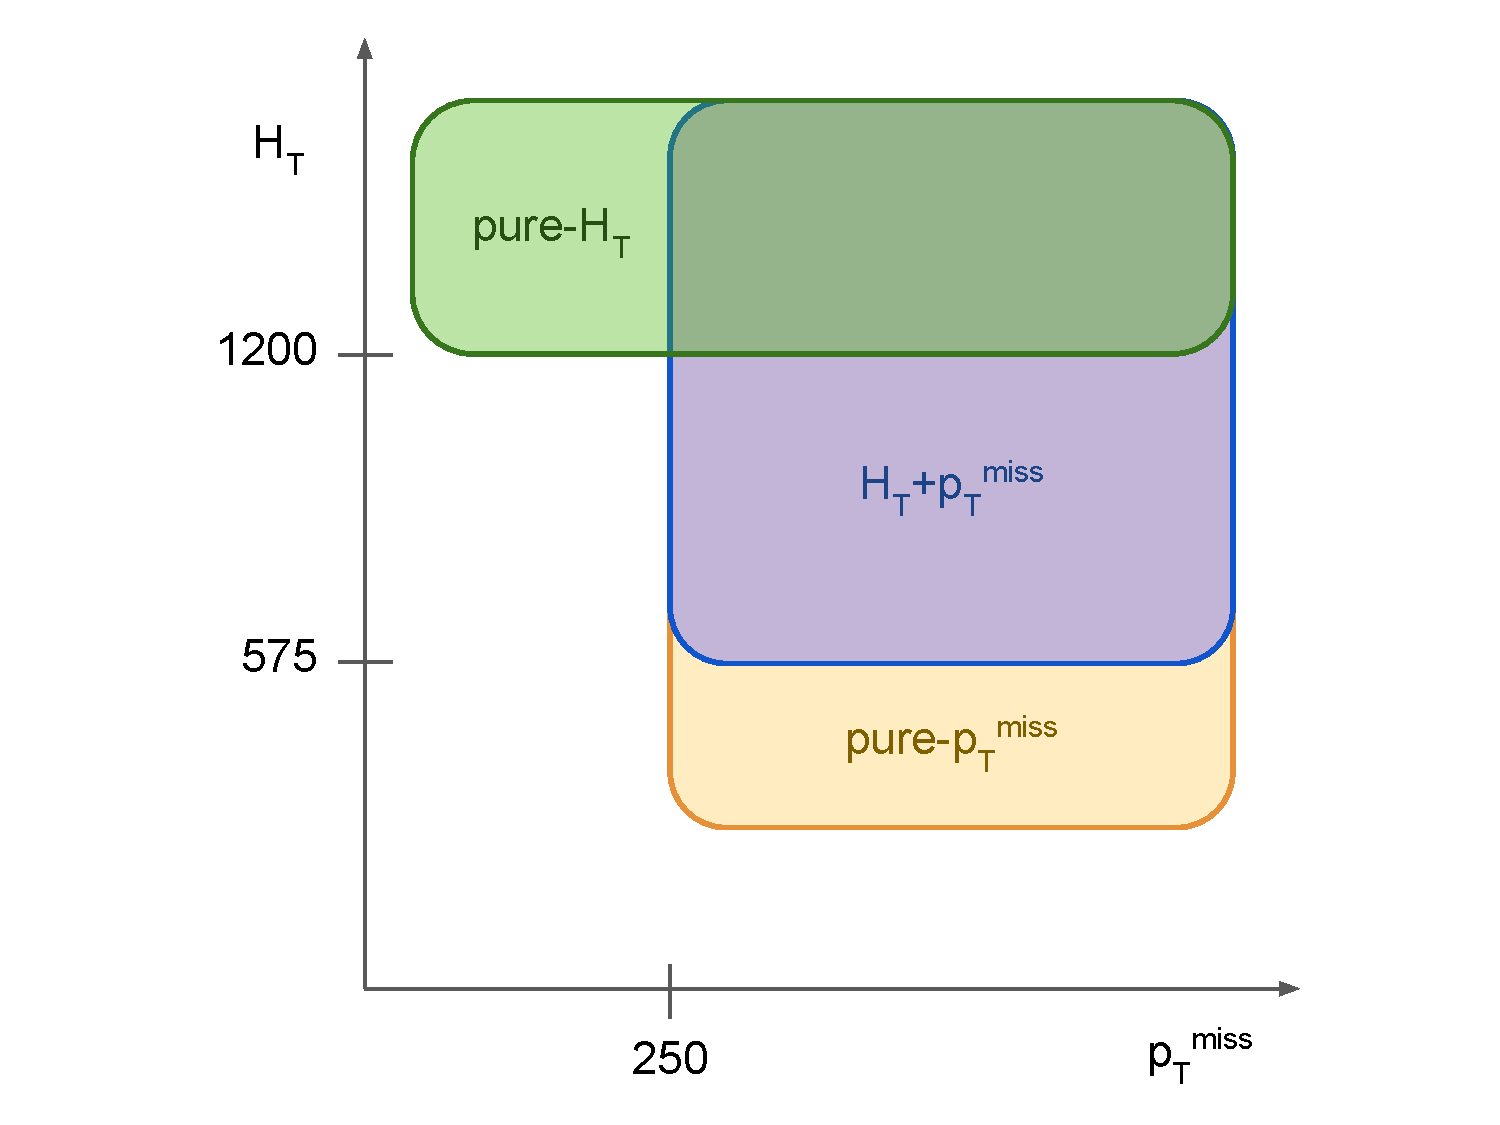
\includegraphics[width=0.65\textwidth]{figs/event_selection/trig_diagram.pdf}
    \caption{Illustration of the trigger coverage of the baseline signal region (defined in Sec.~\ref{sec:baselinesel}).
      The pure-\ptmiss triggers cover the low-\Ht regions, starting at $\ptmiss=250\GeV$.
      The pure-\Ht trigger covers the high-\Ht regions, starting at $\Ht=1200\GeV$.
      The \Ht+\ptmiss triggers provide redundancy and cover for any
      small inefficiencies in the intermediate \Ht regions.
            }
    \label{fig:trig_diagram}
  \end{center}
\end{figure}

Measuring the efficiency of the triggers is imporant to ensure the signal regions are fully covered and trigger
at near 100\%. To make this measurement, a selection in the plateau of an orthogonal ``reference trigger''
is made, and then the efficiency of the desired trigger is plotted as a function of the relevant kinematic
variable. 

The efficiency of the pure-\Ht triggers is measured in two ways: one using an electron trigger
reference, and one using a \ptmiss trigger reference. Both methods start by selecting events that pass
all \ptmiss filter, and that have at least 2 jets with $\pt>30\GeV$ and no leptons (other than the 
potential reference electron). The electron method further requires
that the event passes a single electron trigger, and contains an electron with $\pt>35\GeV$ that is 
isolated and passes a tight cut-based ID. The \ptmiss method requires that the event passes the
pure-\ptmiss trigger and has $\ptmiss>300\GeV$. Both methods give consistent results, with 
pleateau efficiencies of $>$98\%. After combining with the \texttt{HLT\_PFJetXXX} trigger,
the efficiency is $>$99\% in all years. Example measurements are shown in Fig.~\ref{fig:trigmeas_HT}.

\begin{figure}[ht]
  \begin{center}
    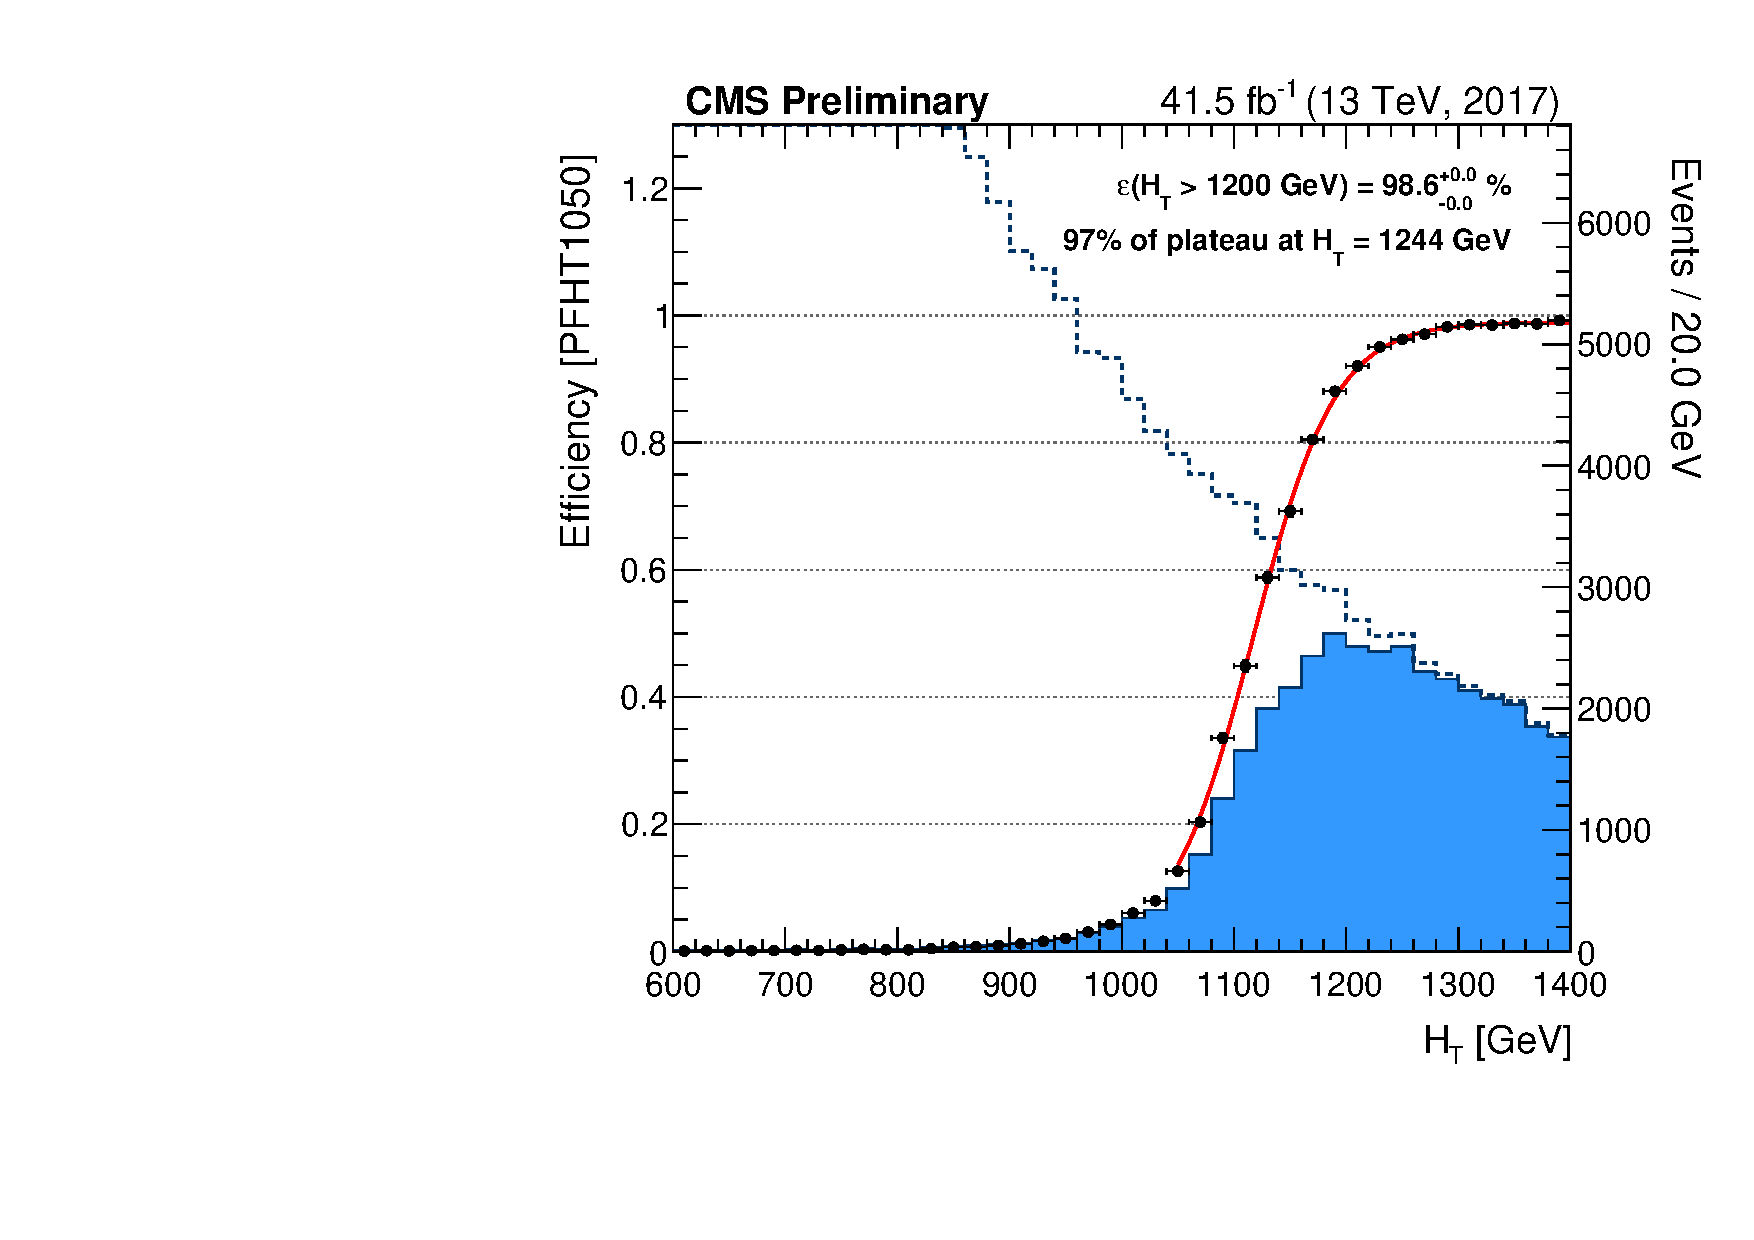
\includegraphics[width=0.49\textwidth]{figs/event_selection/pfht1050_2017_met.pdf}
    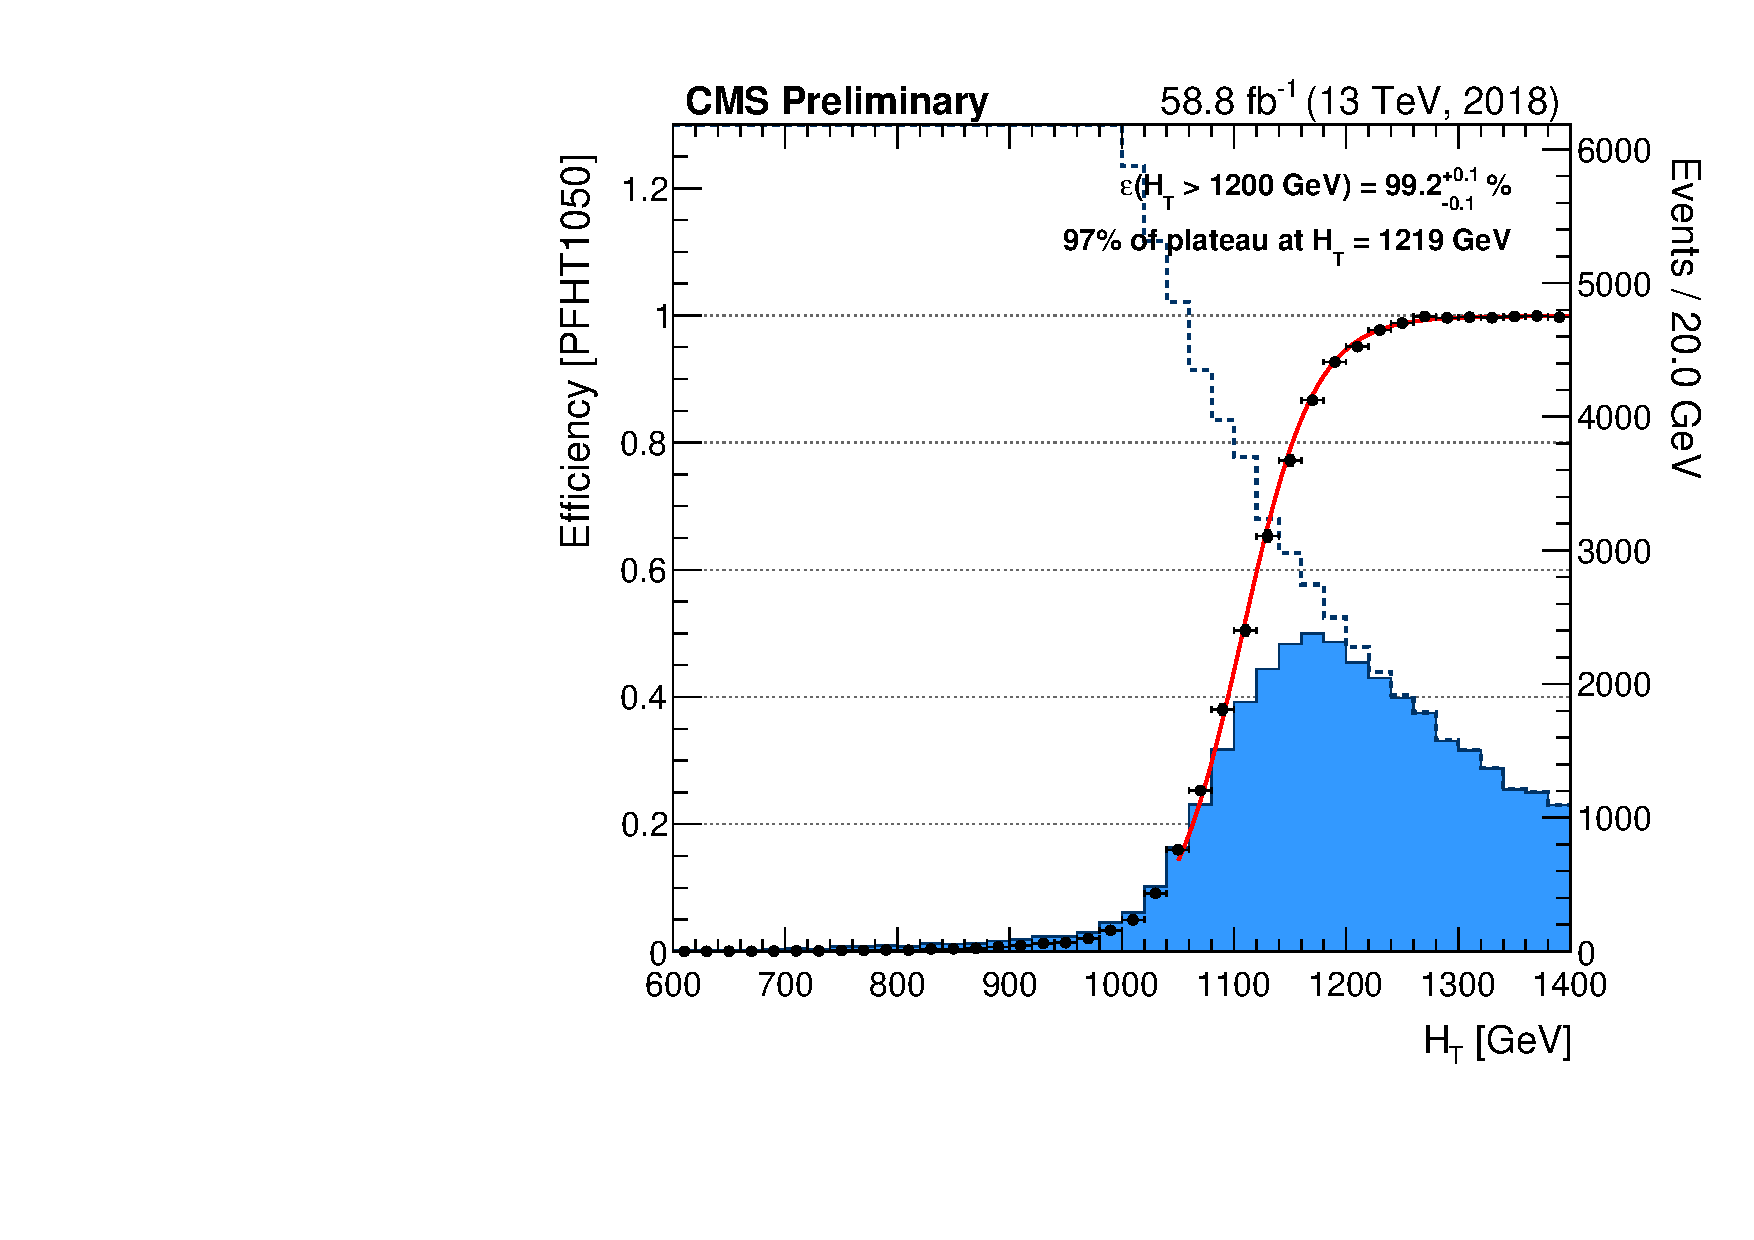
\includegraphics[width=0.49\textwidth]{figs/event_selection/pfht1050_2018_el.pdf}
    \caption{Trigger efficiency measurements for the pure-\Ht \texttt{HLT\_PFHT1050} trigger,
      (left) for 2017 data using a \ptmiss-based reference trigger, and (right) for 2018 data
      using an electron-based reference trigger. The dashed (solid) blue histograms
      are the denominator (numerator) event counts, and the red lines are logistic function fits to the
      efficiency curves.
            }
    \label{fig:trigmeas_HT}
  \end{center}
\end{figure}

The pure-\ptmiss trigger efficiencies are measured using the electron-based method described above.
The \Ht and \ptmiss leggs of the \Ht+\ptmiss triggers must be measured separately. The \Ht leg is measured
using a \ptmiss trigger reference, and the \ptmiss leg is measured using an electron trigger reference
(with the additional requirement of $\Ht>700\GeV$ to ensure that we are in the plateau of the \Ht leg).
Efficiencies of close to 100\% are observed in all cases. Example measurements of the \ptmiss and \Ht+\ptmiss
trigger efficienes are shown in Fig.~\ref{fig:trigmeas_HTMET}.

\begin{figure}[ht]
  \begin{center}
    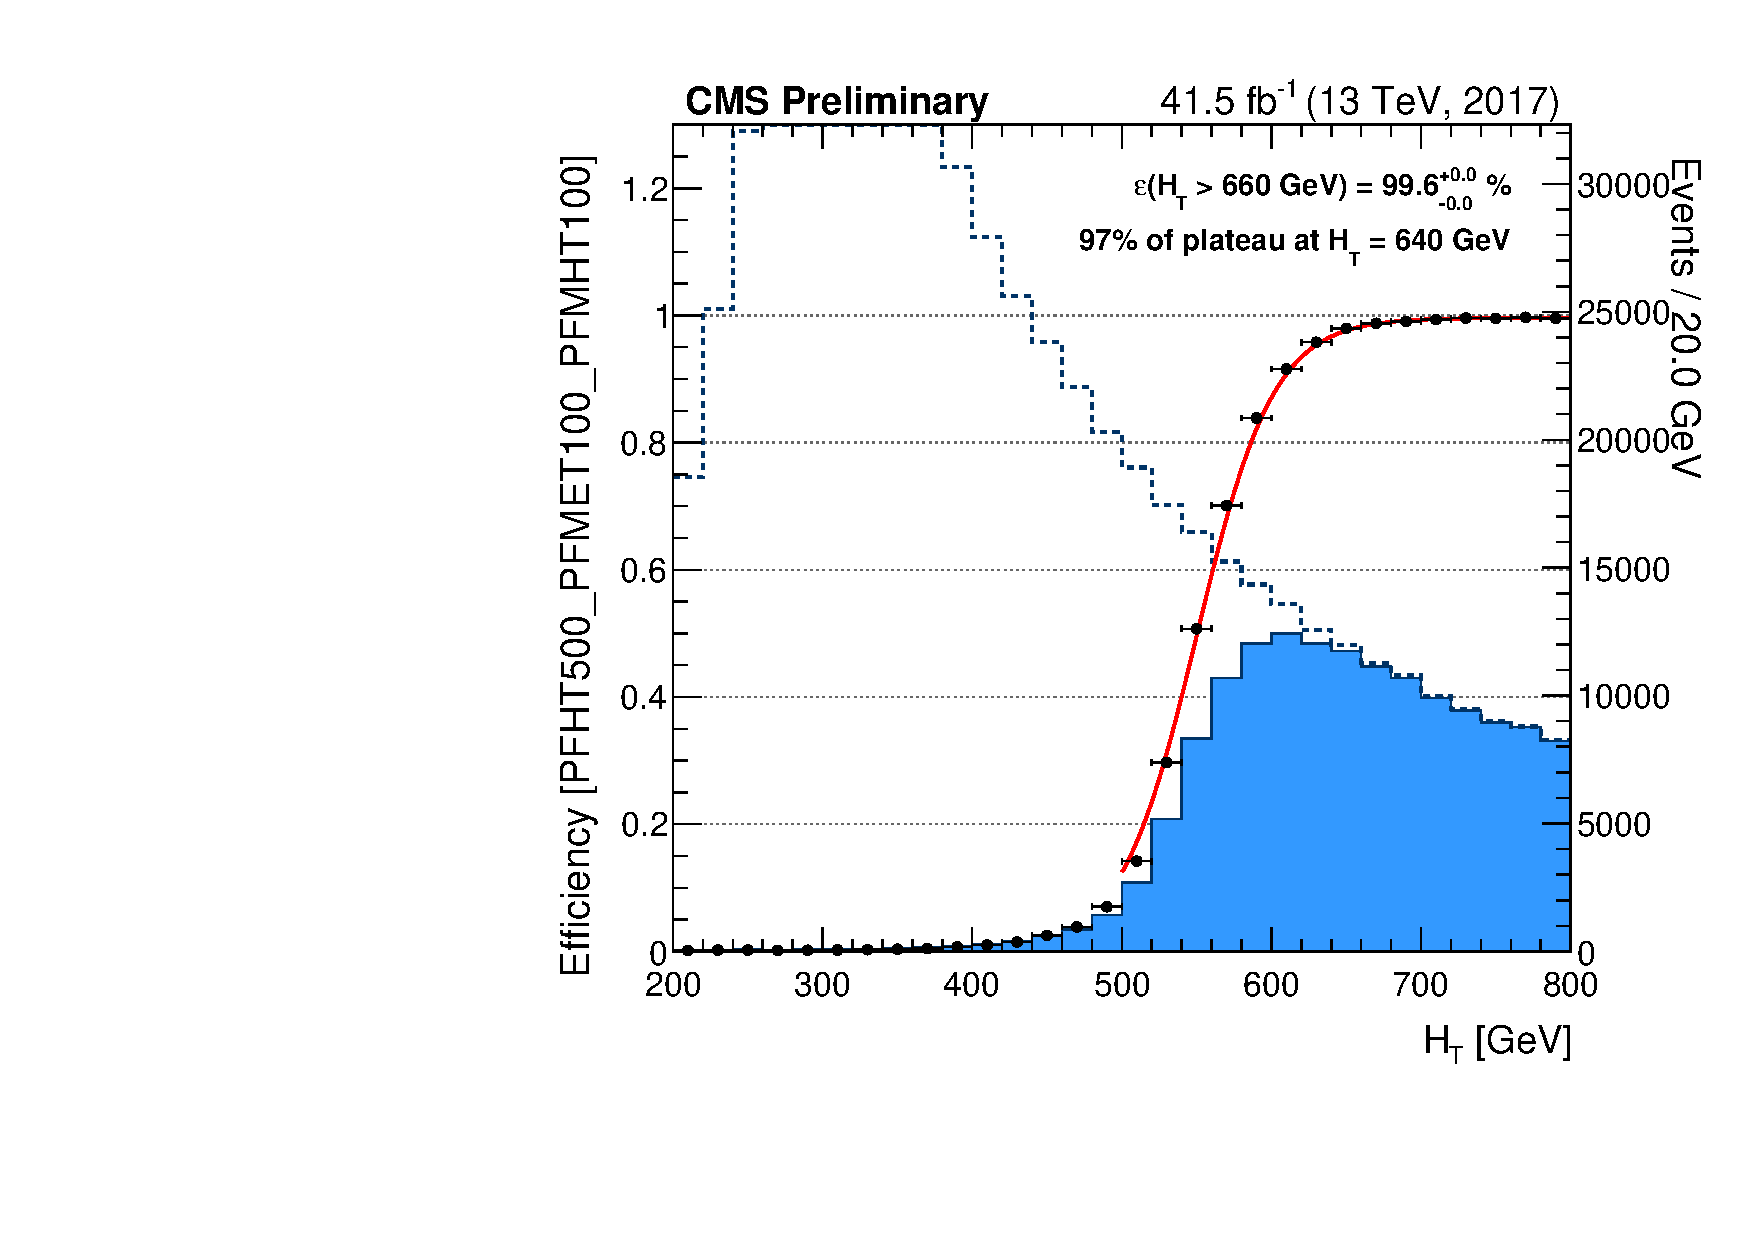
\includegraphics[width=0.49\textwidth]{figs/event_selection/pfht500met100_2017_htleg_met.pdf}
    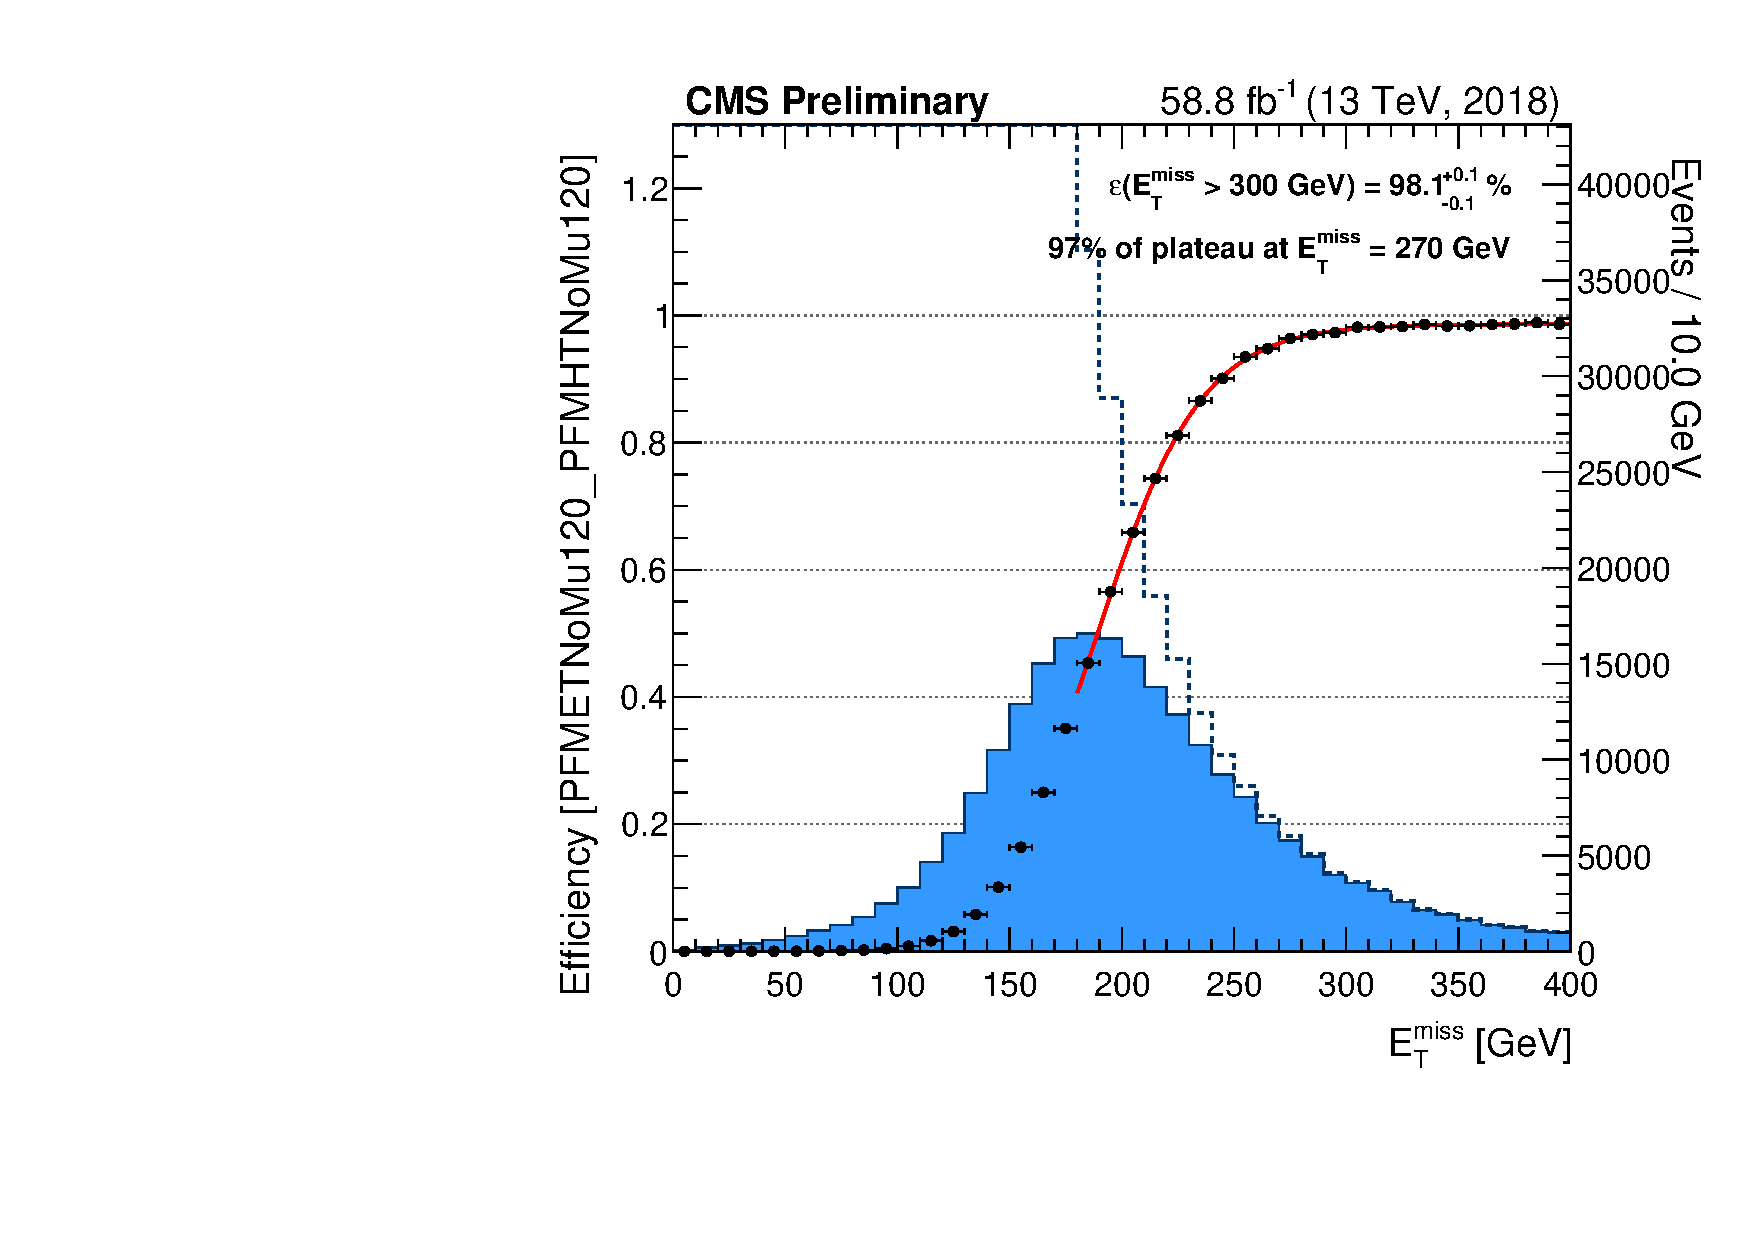
\includegraphics[width=0.49\textwidth]{figs/event_selection/pfmet120nomu_2018_el.pdf}
    \caption{Trigger efficiency measurements (left) for the \Ht-leg of the \texttt{HLT\_PFHT500\_PFMET100}
      trigger in 2017 data, measured with a \ptmiss-based reference trigger, 
      and (right) for the pure-\ptmiss \texttt{HLT\_PFMETNoMu120\_PFMHTNoMu120} trigger
      in 2018 data, measured using an electron-based reference trigger. The dashed (solid) blue histograms
      are the denominator (numerator) event counts, and the red lines are logistic function fits to the
      efficiency curves.
            }
    \label{fig:trigmeas_HTMET}
  \end{center}
\end{figure}

\subsection{Control region triggers}
\label{sec:crtrigs}

Control region definitions are given in Sec.~\ref{sec:crdefs}. Here we only summarize the triggers used,
and it is sufficient to know that there are both single lepton and dilepton control regions used for
predicting the electroweak backgrounds, and an inclusive low-\Ht data sample used in the estimate
of the QCD multijet background.

The single lepton control region is triggered with the same triggers as the signal region, since
the cuts on the relevant kinematic variables are the same (the only difference is the requirement of
exactly one lepton, instead of zero).

This is not true for the dilepton control region, since as we will see the leptons are removed from
the \Ht and added to the \vMet vector before cutting on these variables. So the standard \Ht and
\ptmiss triggers will not work, and special dilepton triggers are used instead.

The dimuon selection is triggered with a combination of isolated and non-isolated
dimuon triggers and non-isolated single-muon triggers (non-isolated and single-muon
paths are to recover inefficiencies at high muon \pt).

Similarly, the dielectron selection is triggered with a combination of isolated and non-isolated
dielectron triggers as well as a single-photon trigger.

Finally, there is an different-flavor (i.e. $e\mu$) control regoin used for estimating \ttbar contamination
in the same-flavor region, that is triggered with a combination of isolated and non-isolated
$e\mu$ triggers, non-isolated single-muon triggers, and a single-photon trigger.

Efficiencies of these dilepton can be measured using pure-\Ht triggers as a reference (both non-prescaled
and lower threshold prescaled triggers).
Plots of measured trigger efficiency as a function of leading and subleading lepton \pt in the relevant
section of phase space are shown in Fig.~\ref{fig:trigmeas_dilep}, for 2017 data. Measurements for 2016 
and 2018 are similar. Inefficiencies up to $\sim10$\% are present; these are accounted for by
applying them as weights to MC on a year-by-year basis as a function of leading and subleading \pt.

\begin{figure}[t]
  \begin{center}
    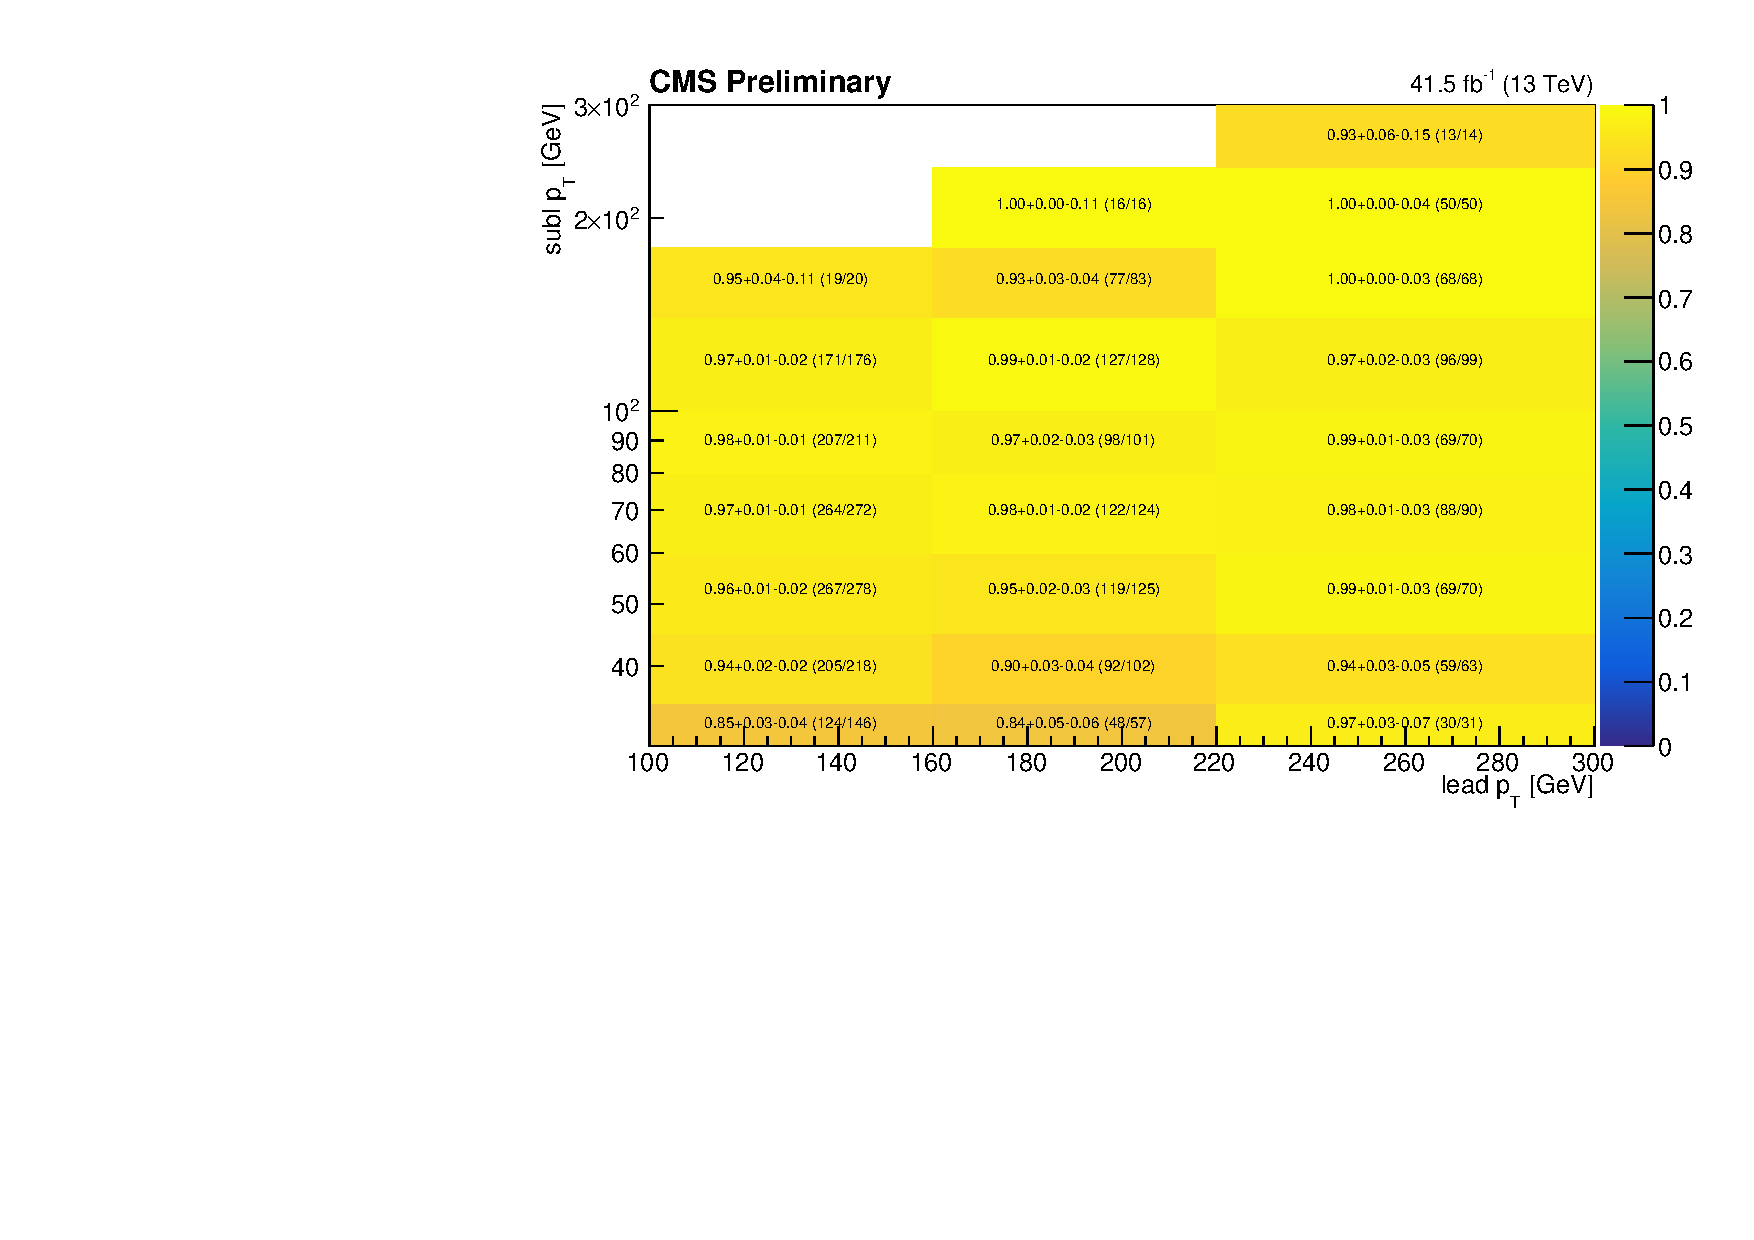
\includegraphics[width=0.49\textwidth]{figs/event_selection/trigeff_dilep_mm_2d_ht_2017fullYear.pdf}
    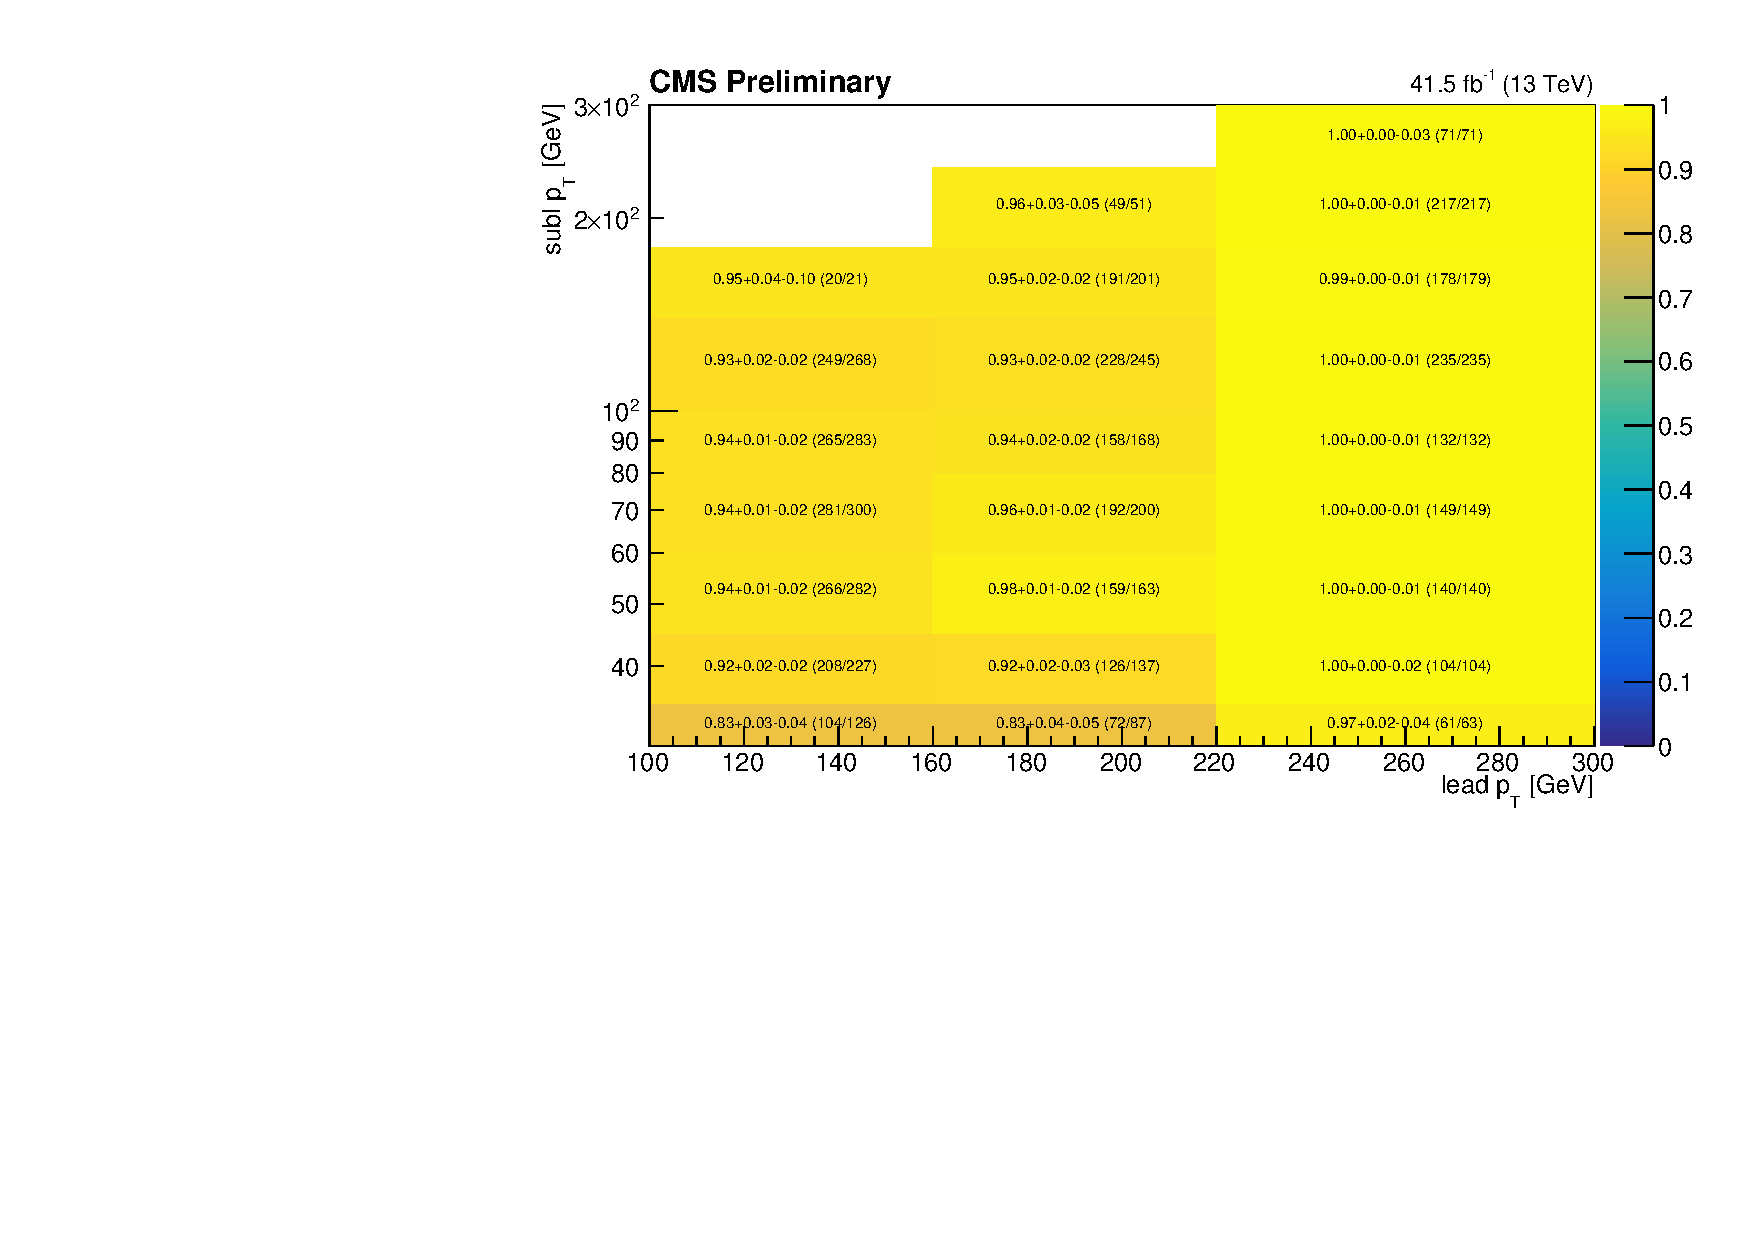
\includegraphics[width=0.49\textwidth]{figs/event_selection/trigeff_dilep_ee_2d_ht_2017fullYear.pdf} \\
    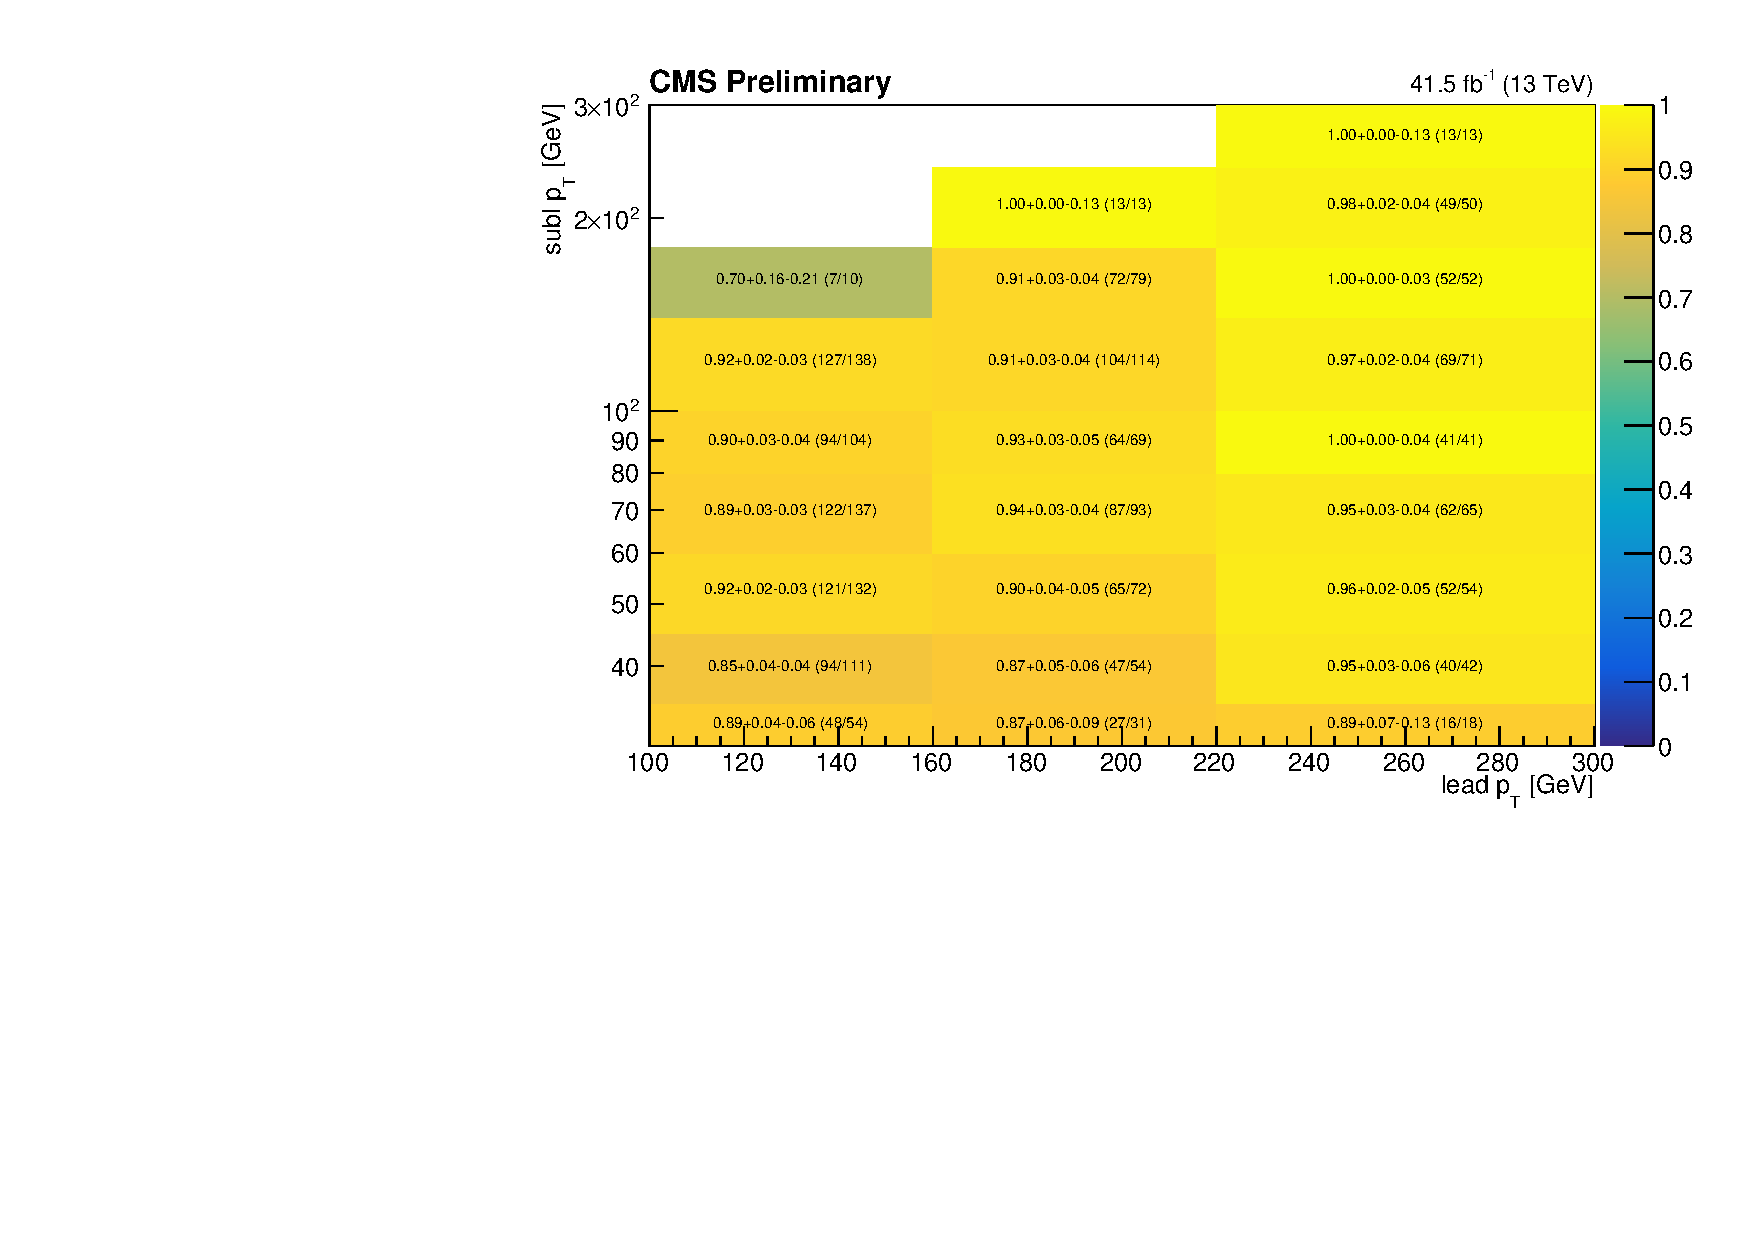
\includegraphics[width=0.49\textwidth]{figs/event_selection/trigeff_dilep_em_2d_ht_2017fullYear.pdf}
    \caption{Measured dilepton trigger efficiences as a function of leading and subleading lepton \pt
      in 2017 data, for (top left) dimuon, (top right) dielectron,
      and (bottom) $e\mu$ selections. Triggers used are a logical OR of the various triggers described
      in Sec.~\ref{sec:crtrigs}. Measurements in 2016 and 2018 are similar.
            }
    \label{fig:trigmeas_dilep}
  \end{center}
\end{figure}

Though not technically a control region, an inclusive selection of low-\Ht events is used in the Rebalance and
Smear method for computing QCD multijet background, described in Chapter~\ref{chap:qcd}. This selection
makes use of low-threshold pure-\Ht triggers, that are necessarily prescaled due to their very
high rates. Though event-by-event prescale values are stored in the data (the exact prescale rate
depends on the instantaneous luminosity and the exact trigger menu being used, so vary with time),
yearly ``effective prescales'' are measured as a constistency check. This is done by measuring the
ratio of rates of different triggers as a function of \Ht, and fitting the ratio
in the plateau. Comparing to the high threshold unprescaled trigger, the effective prescales of
all others can be determined.

A plot measuring the effective prescales in 2017 data is shown in Fig.~\ref{fig:pureht_prescales} (left).
On the right is the observed \Ht spectrum using these prescale values, which is smooth as
is expected if the correct prescales are measured.

\begin{figure}[t]
  \begin{center}
    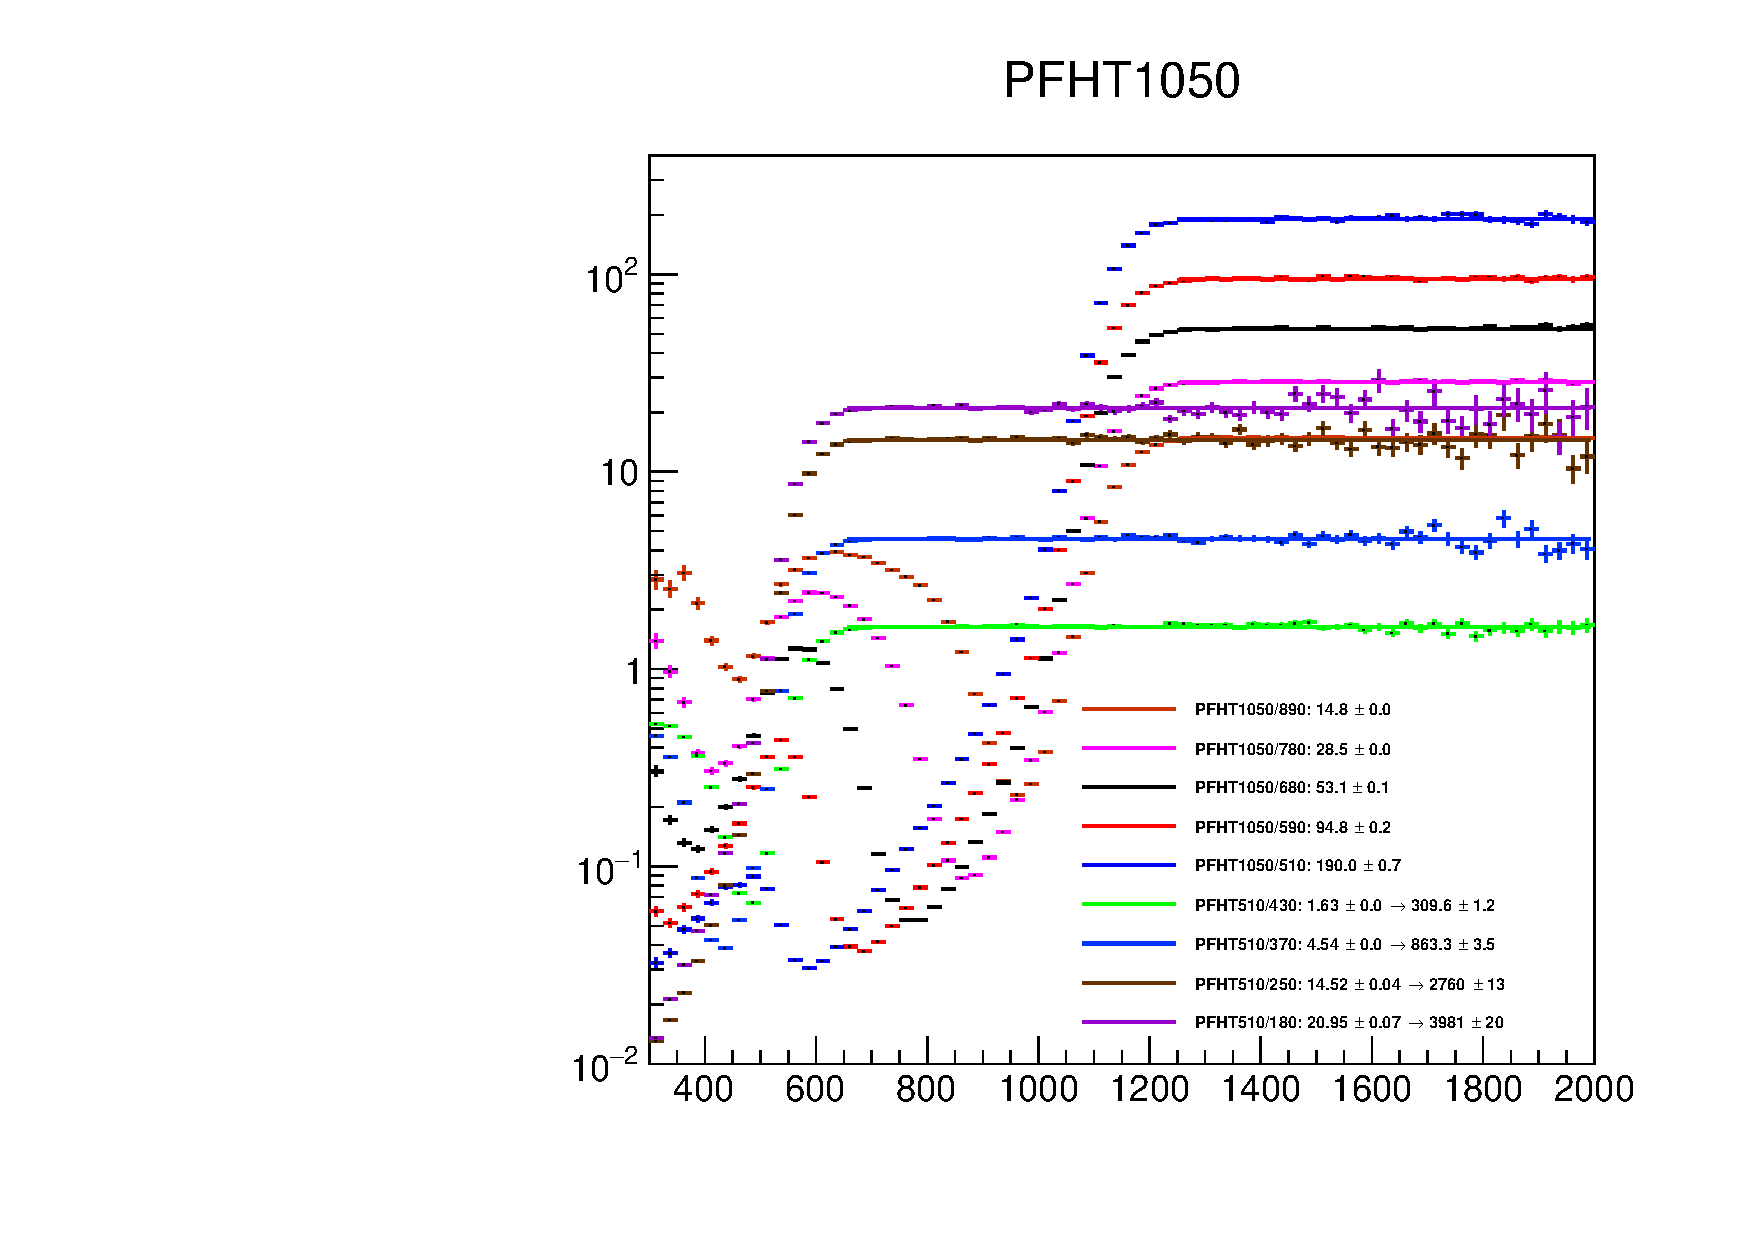
\includegraphics[width=0.45\textwidth]{figs/event_selection/prescales_2017.pdf}
    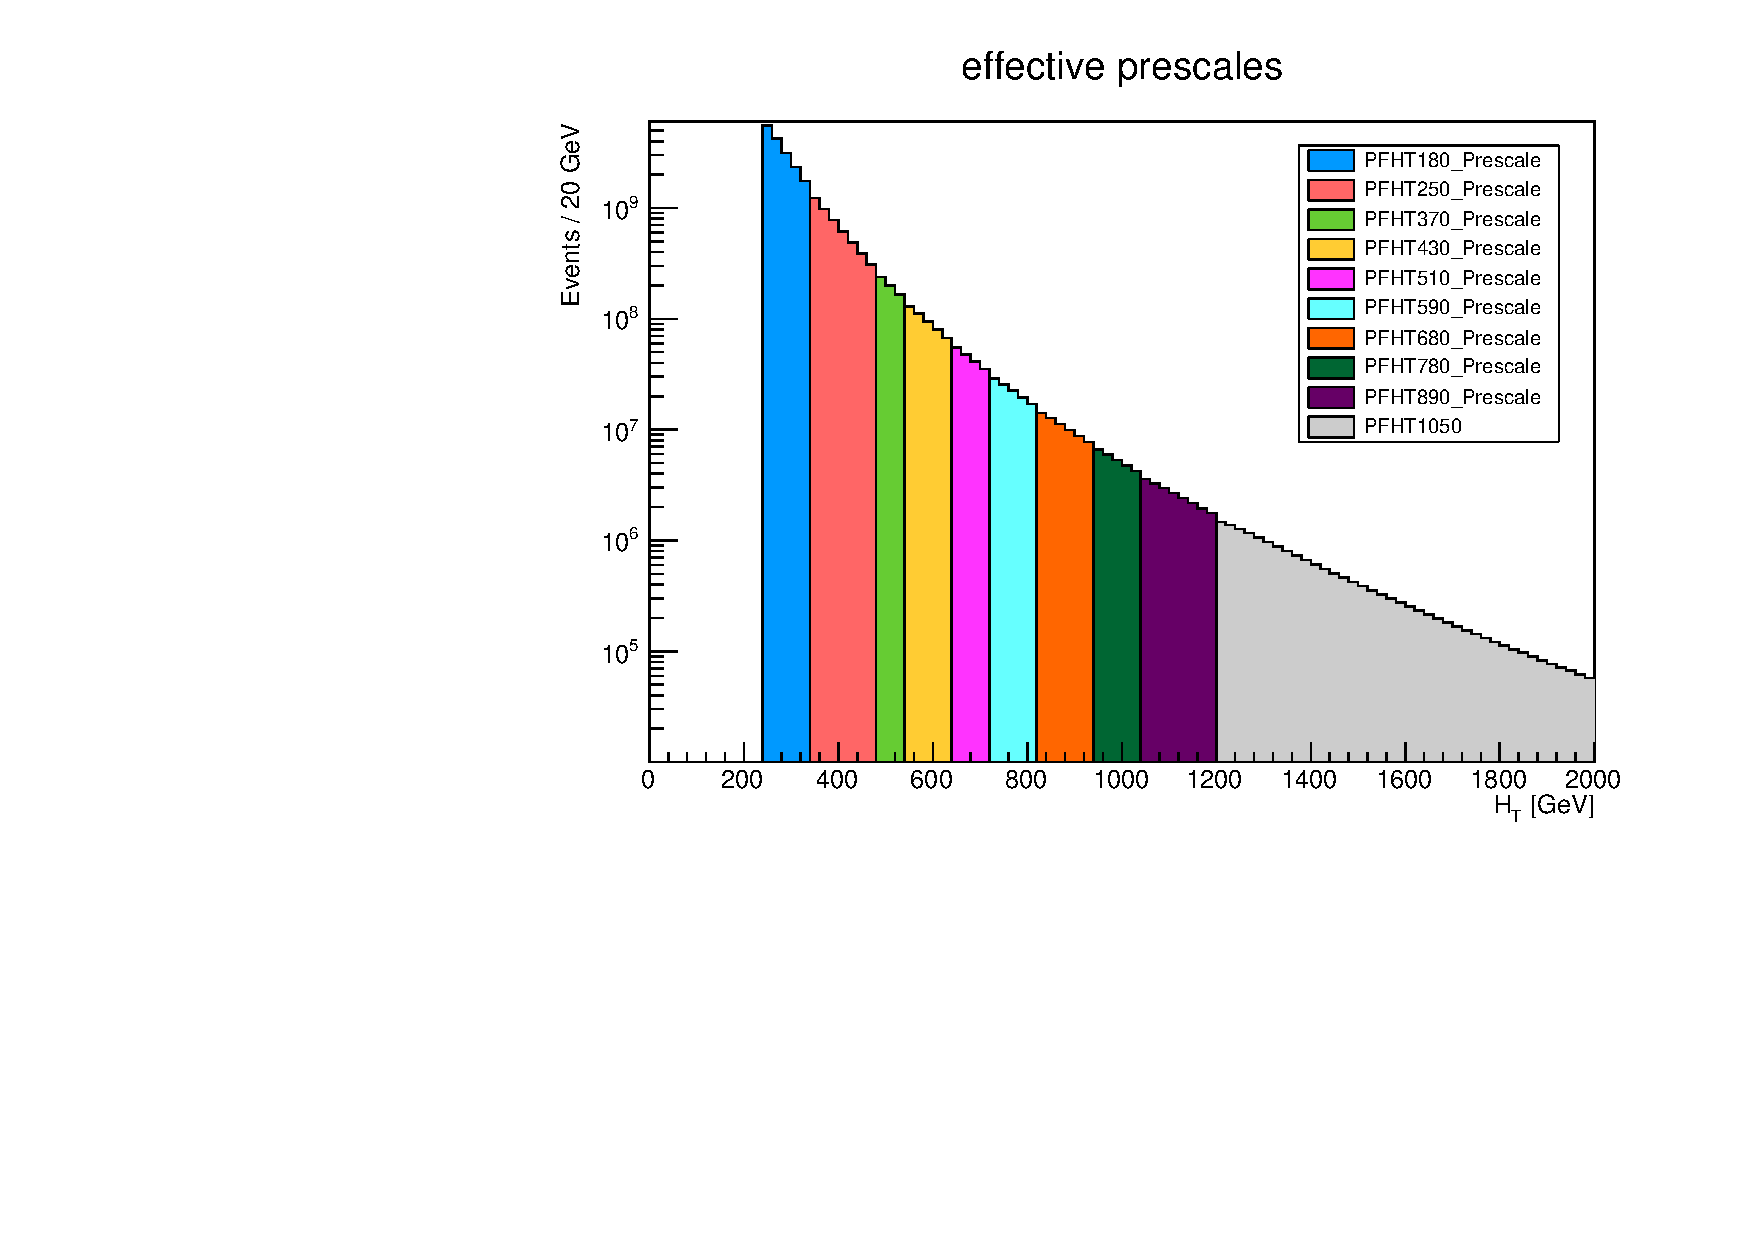
\includegraphics[width=0.54\textwidth]{figs/event_selection/htSpect2017_meth1.pdf} \\
    \caption{(left) A plot of the ratio of rates of various pure-\Ht triggers in
      2017 data. The value at the plateau gives the relative prescale between two triggers,
      and comparing to the unprescaled \texttt{HLT\_PFHT1050} gives the absolute prescale.
      (right) The observed \Ht spectrum using these prescales, which is smooth as is expected 
      if the correct values are measured.
            }
    \label{fig:pureht_prescales}
  \end{center}
\end{figure}

\section{Baseline selection}
\label{sec:baselinesel}

Using the object and variable definitions detailed in Sec.~\ref{sec:objvardefs}, the
baseline selection used for all analysis signal regions is as follows:
\begin{itemize}\setlength\itemsep{-1mm}
\item at least one good vertex, as defined in Sec.~\ref{sec:vertices}
\item pass all \ptmiss filters, as defined in Sec.~\ref{sec:metfilters}
\item pass the logical OR of all signal region triggers listed in Sec.~\ref{sec:srtrigs}
\item $\Ht>1200\GeV$ and $\ptmiss>30\GeV$, or $\Ht>250\GeV$ and $\ptmiss>250\GeV$. These cuts are
based on the available trigger thresholds, and illustrated in Fig.~\ref{fig:trig_diagram}.
\item $\dphimet>0.3$. This protects against large \ptmiss from jet mis-measurement in multijet events,
and rejects a large fraction of QCD background.
\item $|\vMht-\vMet|/\ptmiss<0.5$. This requires that \vMht be similar to \vMet, and in doing so
protects agains bias in the shape of \mttwo. \ptmiss is sensitive to reconstructed objects with
$\pt<30\GeV$ or $|\eta|>2.4$, where as these are not used in \vMht or in the construction of
pseudojets for \mttwo, so a large contribution from these objects to the missing transverse energy
can bias the \mttwo distribution.
\item lepton veto: to reduce the background from events with a $W$ boson decay, we reject events if they contain
\vspace{-\topsep}
\begin{itemize}\setlength\itemsep{-1mm}
\item a reconstructed electron or muon as defined in Secs.~\ref{sec:electrons} and \ref{sec:muons}
\item a particle-flow electron, muon, or hadron candidate as defined in Sec.~\ref{sec:isotracks},
with the additional requirement of $M_\mrm{T}(\mrm{cand},\vMet)<100\GeV$ (to avoid vetoing
signal events, which contain \ptmiss not from the leptonic $W$ decay and hence have high $M_\mrm{T}$).
\end{itemize}
\item $\mttwo>200\GeV$ (only for events with at least 2 jets). This provides a large rejection of QCD
multijet events that have large \ptmiss from mis-measured jets, as discussed in Sec.~\ref{sec:mt2_variable}.
The threshold is raised to $\mttwo>400\GeV$ for events with $\Ht>1500\GeV$, in order to ensure that
QCD multijet events remain a subdominant background.
\end{itemize}

\section{Signal region definitions}
\label{sec:srdefs}

After the baseline selection defined in Sec.~\ref{sec:baselinesel}, signal regions are further categorized
into different bins of \Ht, \Nj, \Nb, and \mttwo.

First, we categorize $\Nj\geq2$ (multijet) events by \Ht, \Nj, and \Nb. Each $(\Ht,\Nj,\Nb)$ bin is referred to as a
\emph{topological region}.
\begin{itemize}\setlength\itemsep{-1mm}
\item Five \Ht regions: $[250,450],[450,575],[575,1200],[1200,1500],[1500,\infty]$\GeV.
These bins are referred to here and throughout this dissertation as Very Low, Low, Medium,
High, and Extreme \Ht, respectively.
\item For the first three \Ht regions, we use 11 bins in \Nj and \Nb:
\vspace{-\topsep}
\begin{itemize}\setlength\itemsep{-1mm}
\item 2--3 jets; 0, 1, 2 b tags
\item 4--6 jets; 0, 1, 2 b tags
\item 2--6 jets; $\geq$3 b tags
\item $\geq$7 jets; 0, 1, 2, $\geq$3 b tags
\end{itemize}
\item For the highest two \Ht regions, we further subdivide the $\Nj\geq7$ regions
for a total of 17 bins in \Nj and \Nb:
\vspace{-\topsep}
\begin{itemize}\setlength\itemsep{-1mm}
\item 2--3 jets; 0, 1, 2 b tags
\item 4--6 jets; 0, 1, 2 b tags
\item 2--6 jets; $\geq$3 b tags
\item 7--9 jets; 0, 1, 2, 3, $\geq$4 b tags
\item $\geq$10 jets; 0, 1, 2, 3, $\geq$4 b tags
\end{itemize}
\end{itemize}

The division into topological regions for the High \Ht region is shown in Fig.\ref{fig:piechart_H}, along
with background composition in each region. We see that QCD multijet background becomes more important with
increasing \Nj, and top background becomes more dominant with increasing \Nb.

\begin{figure}[t]
  \begin{center}
    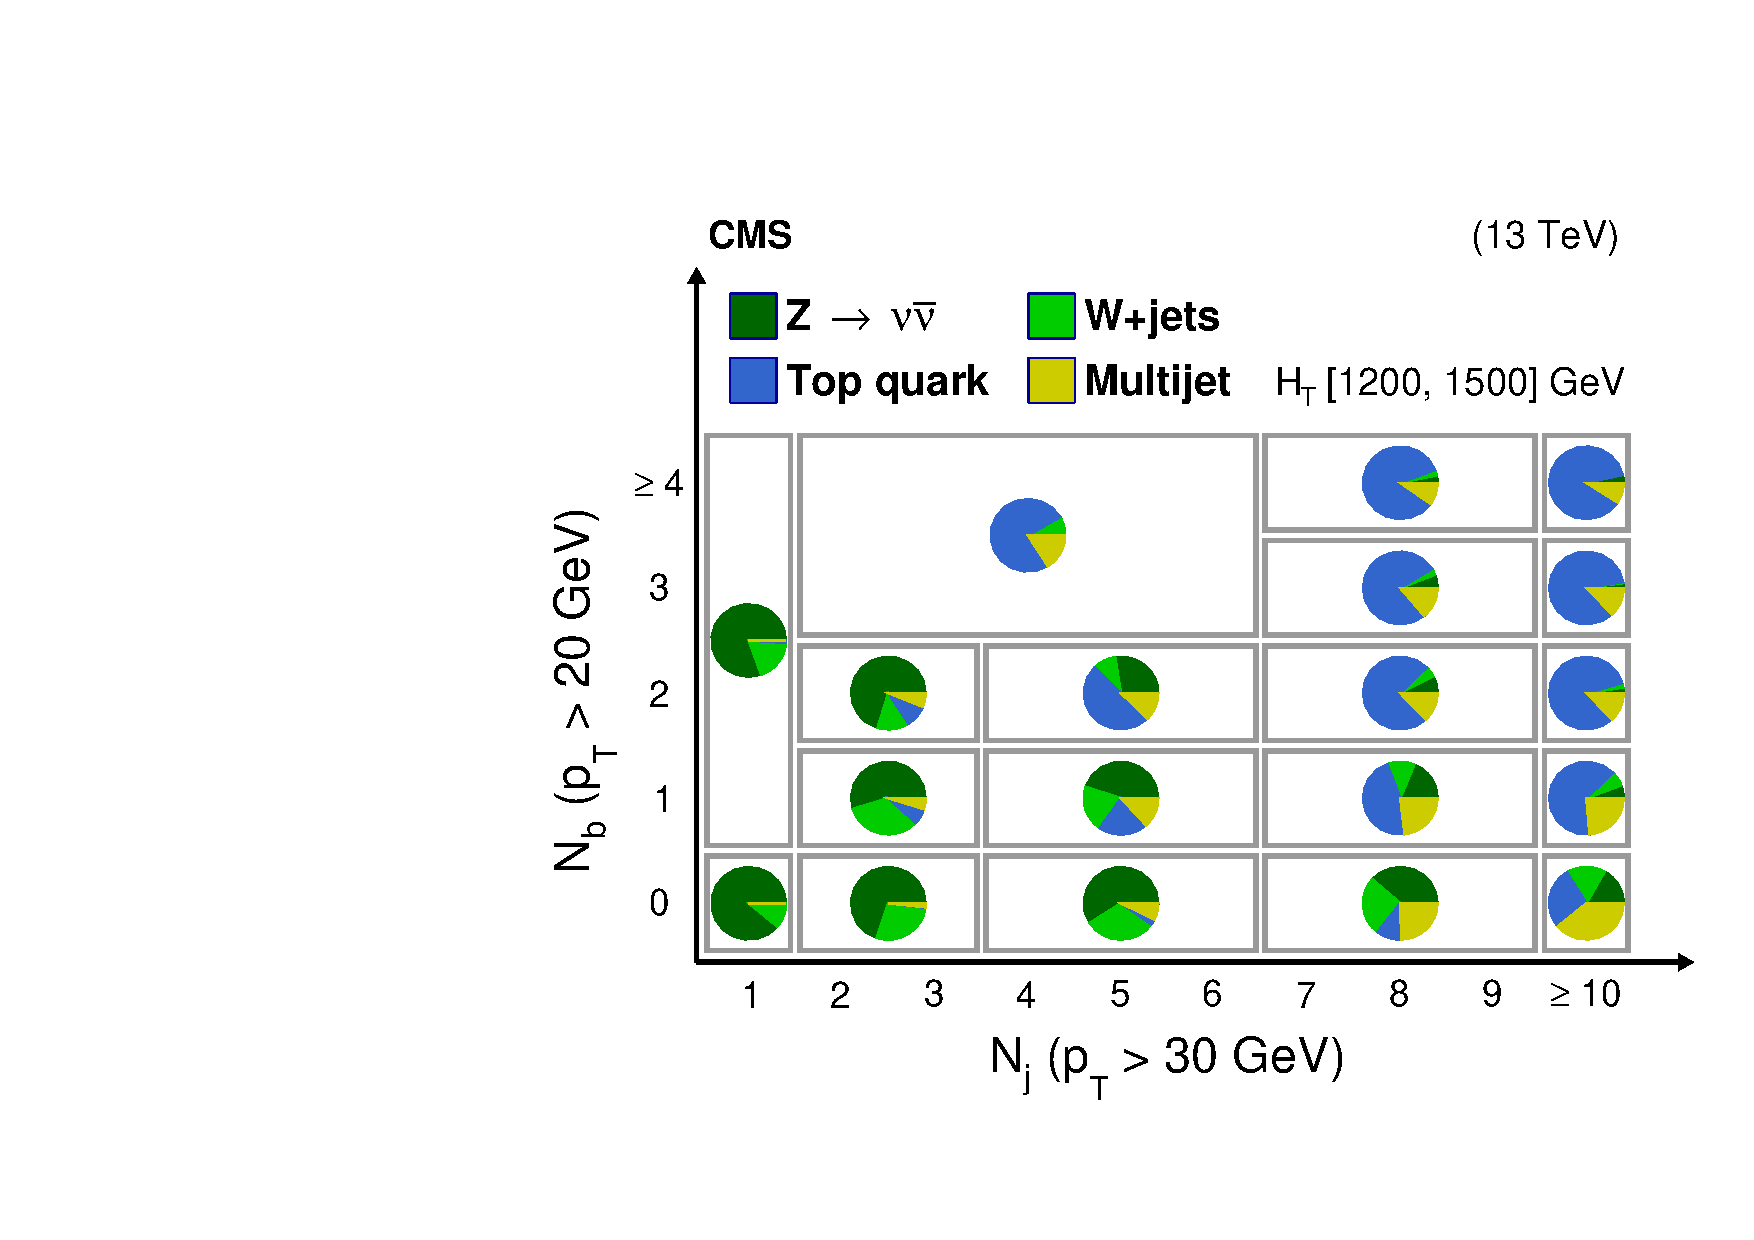
\includegraphics[width=0.8\textwidth]{figs/event_selection/piecharts_H.pdf}
    \caption{Topological region binning (defined by the solid gray lines)
      for the High \Ht region ($1200\leq\Ht<1500\GeV$). The proportion
      of each background type is shown as a pie chart in each topological region. QCD multijet becomes more imporant
      with increasing \Nj, and top backgrounds become more dominant at high \Nb. Background composition is estimated
      using the data-driven techniques described in the following chapters.
            }
    \label{fig:piechart_H}
  \end{center}
\end{figure}

Finally, we further divide each topological region into bins of \mttwo. The bin thresholds are chosen according
to the following criteria:
\begin{itemize}\setlength\itemsep{-1mm}
\item The lower edge of the first \mttwo bin is 200\GeV, except for $\Ht>1500$\GeV (Extreme \Ht) where it is 400\GeV.
\item In each topological region, we select the lower threshold of the last \mttwo bin such that this
bin is expected, from simulation, to contain approximately one background event. Moreover, the upper limit on \Ht
effectively places an upper limit on \mttwo. Therefore, this lower \mttwo threshold should not be larger than the upper limit
on \Ht, in each \Ht region.
\item Bin widths are nominally chosen to be 100\GeV. In each topological region, we merge \mttwo bins which are 
expected to contain less than one background event. In a few cases, we merge intermediate \mttwo bins
to minimize the number of signal region bins.
\end{itemize}

The final \mttwo binning for the multijet search regions can be found in 
Tables~\ref{tab:yieldsVL} through \ref{tab:yieldsUHh} in Appendix~\ref{app:yield_tables}

In addition to the $\Nj\geq2$ bins described above, we also select events with $\Nj=1$ (monojet), with the jet required to have
$\pt(\mrm{jet})>250\GeV$. Events are then categorized as follows:
\begin{itemize}\setlength\itemsep{-1mm}
\item Two \Nb regions: $\Nb=0$ and $\Nb\geq1$ (since the \pt threshold for \Nb is lower than that for \Nj, it
is possible that $\Nb>1$ even when $\Nj=1$)
\item For $\Nb=0$, \Ht bin edges of $[250,350,450,575,700,1000,1200,\infty]$\GeV
\item For $\Nb\geq1$, \Ht bin edges of $[250,350,450,575,700,\infty]$\GeV
\end{itemize}

In total, there are 270 multijet and 12 monojet regions for a total of 282 signal region search bins.

\section{Control regions}
\label{sec:crdefs}

To estimate the various backgrounds for this analysis, we make use of a number of control regions orthogonal 
to the signal region. These include a single lepton selection, a dileptonic selection (mostly \zll events), 
and a selection enriched in QCD multijet events.

\subsection{Single lepton control region}
\label{sec:crsl}
A single lepton selection is used to esimate backgrounds from \ttbar and \wjets (``lost lepton'' background).
The selection is the same as the baseline selection described in Sec.~\ref{sec:baselinesel}, with
the exception of the lepton veto. Instead, we require exactly one candidate passing the reconstructed lepton
or particle-flow lepton selections ($e$ or $\mu$ only). We further require this lepton candidate to satisfy
$M_\mrm{T}(\mrm{cand},\ptmiss)<100\GeV$ to reduce signal contamination. Events in which both the lepton
and missing energy are from leptonic $W$ decay tend to have $M_\mrm{T}\lesssim M_W=80\GeV$, while signal
events (in which the predominant source of \ptmiss is \emph{not} $W$ decay) tend to have much larger $M_\mrm{T}$.
As the \Ht and \ptmiss selections are the same as in the baseline signal region selection, 
the same triggers as used in the signal region are used for this single lepton control region.

When a true lepton is within detector acceptance, it is generally reconstructed in some form, even if
not classified as an isolated lepton candidate. We therefore remove the closest jet within
$\Delta R<0.4$ of the lepton candidate and count the lepton as a visible object for the purpose of computing
the variables \Ht, \Mht, \dphimet, $|\vMht-\vMet|/\ptmiss$, and \mttwo. The lepton is \emph{not} however used
in computing \Nj, as most leptons have low \pt.

The baseline single lepton control region is separated into $(\Ht,\Nj,\Nb)$ topological regions
in the same way as the signal region, with the exception of events with $\Nj\geq7$.
The regions with $\geq$7 jets and $\geq$1 b tag are all predicted using control region bins with 7--9 or $\geq$10 jets and 1--2 b tags
(but with the same \Ht binning as the signal regions).
This is motivated by the low control region statistics in bins with $\geq$10 jets or $\geq$7 jets and $\geq$2 b tags,
as well as potential signal contamination in bins with $\geq$7 jets and $\geq$3 b tags.
Similarly, regions with either 7--9 or $\geq$10 jets and 0 b tags are all predicted using control region bins
with $\geq7$ jets and 0 b tags, due to low control region statistics in bins with $\geq$10 jets.

The single lepton control region is not binned in \mttwo like the signal regions. Instead, the lost
lepton prediction along the \mttwo dimension is estimated using a hybrid technique described in 
Chapter~\ref{chap:lostlep}.

\subsection{Dilepton control regions}
\label{sec:dilep_cr}
We make use of two dilepton control regions: a same-flavor $e^\pm e^\mp/\mu^\pm\mu^\mp$ control region, consisting mostly
of \zll events and used to estimate the \znunu background, and an different-flavor $e^\pm\mu^\mp$
control region, used to estimate contamination from flavor-symmetric processes (mainly \ttbar)
in the same-flavor region.

In either case, we require two opposite-charge leptons passing the reconstructed lepton selections
given in Secs.~\ref{sec:electrons} and \ref{sec:muons}. Dileptonic triggers are used, 
and to improve trigger efficiency we further
require that electrons pass a slightly tigher cut-based ID requirement (``loose'' instead of ``veto'').
The leptons must satisfy $\pt(\ell\ell)>200\GeV$ (to ensure similar kinematics to high-\pt \znunu
events that populate the signal regions), and leading/subpleading lepton $\pt>100/35\GeV$. The invariant
mass $m_{\ell\ell}$ must satisfy $|m_{\ell\ell}-m_Z|<20\GeV$ in order to ensure we select mainly $Z$ events.

Since the leptons take the place of the neutrinos in \znunu events, to emulate the kinematics the
lepton \vSS{p}{T}{} vectors are added to the \vMet vector for use in the computation of all
kinematic variables. Further, since leptons are usually reconstucted as (at least components of) jets,
the closest jet within $\Delta R<0.4$ of each lepton is removed from the event before computing kinematic
quantities. The variables \Nj, \Nb, \Ht, \Mht, \dphimet, $|\vMht-\vMet|/\ptmiss$, and \mttwo are all
potentially modified by these changes.

In addition to the main same-flavor and different-flavor control regions described above, there is
additionally an auxilliary different-flavor region enriched in \ttbar, used to measure the ratio
of same-flavor to different-flavor events from flavor-symmetric processes. This is defined by
inverting the $\pt(\ell\ell)$ and $m_{\ell\ell}$ selections, so that $\pt(\ell\ell)<200\GeV$
and $|m_{\ell\ell}-m_Z|>20\GeV$.

Similarly as for the single lepton control region, the dilepton control region is binned into
topological in the same way as the signal region, with the exception of bins with $\geq$7 jets.
This time, signal regions with 7--9 or $\geq$10 jets and 0 b tags are predicted with control
region bins with $\geq$7 jets and 0 b tags, and signal regions with 7--9 or $\geq$10 jets and
$\geq$ 1 b tag are predicted using control regions with $\geq$ 7 jets and $\geq$ 1 b tag
(still with the same \Ht binning as the signal regions).

\subsection{QCD-enriched control regions}
We define a few control regions orthogonal to the signal region that are enriched in
QCD multijet events, in order to validate the estimate of the QCD multijet background.
This is done by inverting cuts on the two kinematic variables mainly responsible for
rejecting QCD background. The baseline signal region selection is applied, with the
exception of one of the following:
\begin{itemize}\setlength\itemsep{-1mm}
\item the \dphimet requirement is inverted to $\dphimet<0.3$.
\item the \mttwo requirement is shifted to $100<\mttwo<200\GeV$
\item \emph{both} the \dphimet and \mttwo cuts are changed as above
\end{itemize}
%
The same triggers are used as in the signal regions.

\section{2018 HEM-15/16 failure}
\label{sec:hem}

During 2018 data taking, two modules in the minus-side HCAL endcap (HEM), 
representing about a 45$^\circ$ angle, were lost.
This means that any energy deposited in these modules was not recorded.
The effects of this are (1) under-measured jets in the region,
as a fraction of the energy is lost, and (2) increased electron and
photon fake rates, as jets in the region have inflated EM-to-hadronic
energy ratios.

Studies showed this has negligible impact on backgrounds with real \ptmiss
(i.e. invisible $Z$ and lost lepton), but a significant effect
on the fake-\ptmiss QCD multijet background.  Fig.~\ref{fig:hem} shows
on the left the actual observed effect on an imbalanced dijet control region,
and on the right the estimated effect on QCD yields in the signal regions,
found by modifying the Rebalance \& Smear method with special HEM response
functions measured in HEM-emulated data. Up to an 8-fold increase in QCD
background is observed.
Additionally, we observed an excess of events in the single lepton
control region with the single lepton being a fake electron in the HEM region.

To avoid contaminating our signal and control regions with these HEM-affected events,
we apply a special veto to the affected portion of 2018 data,
as well as a fraction of the 2018 MC events corresponding to the
fraction of affected data (about 39 out of 58 fb$^{-1}$, or 66\%).
The filter rejects events containing certain objects in the HEM region, defined
as $\eta\in[-4.7,-1.4]$ and $\phi\in[-1.6,-0.8]$.
The objects that trigger the veto are as follows:
\begin{itemize}\setlength\itemsep{-1mm}
\item For events with $\Nj=1$ or $\Ht<575\GeV$, any jet with $\pt>20\GeV$.
\item Also for events with $\Nj=1$ or $\Ht<575\GeV$, any lost track with $d_z<0.2$ cm
and $d_{xy}<0.1$ cm (a ``lost track'' is any track not reconstructed as a PF candidate).
\item For events with $\Nj\geq2$ and $\Ht\geq575\GeV$, any jet with $\pt>30\GeV$.
\item The electron for any events in the single lepton control region.
\end{itemize}

\begin{figure}[t]
  \begin{center}
    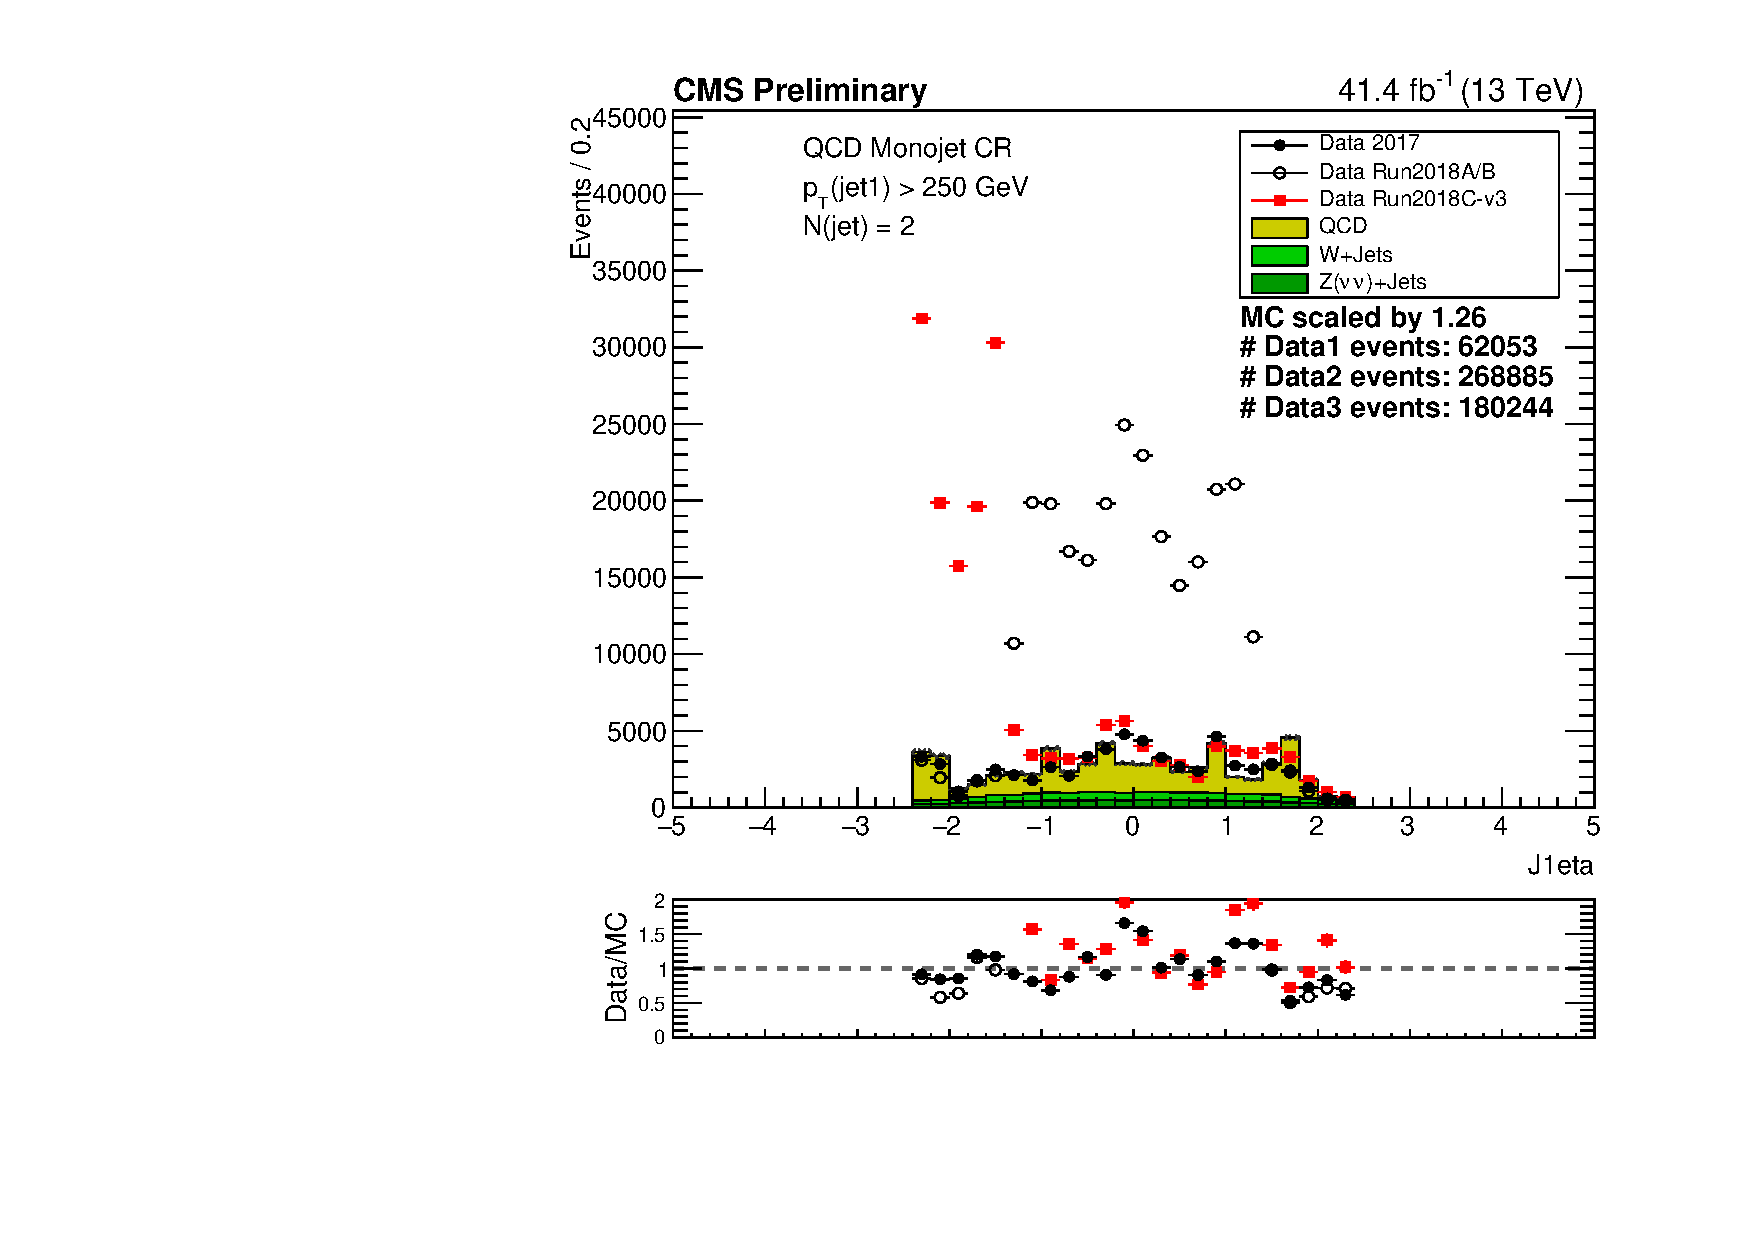
\includegraphics[width=0.48\textwidth]{figs/event_selection/hem_subleadjeteta.pdf}
    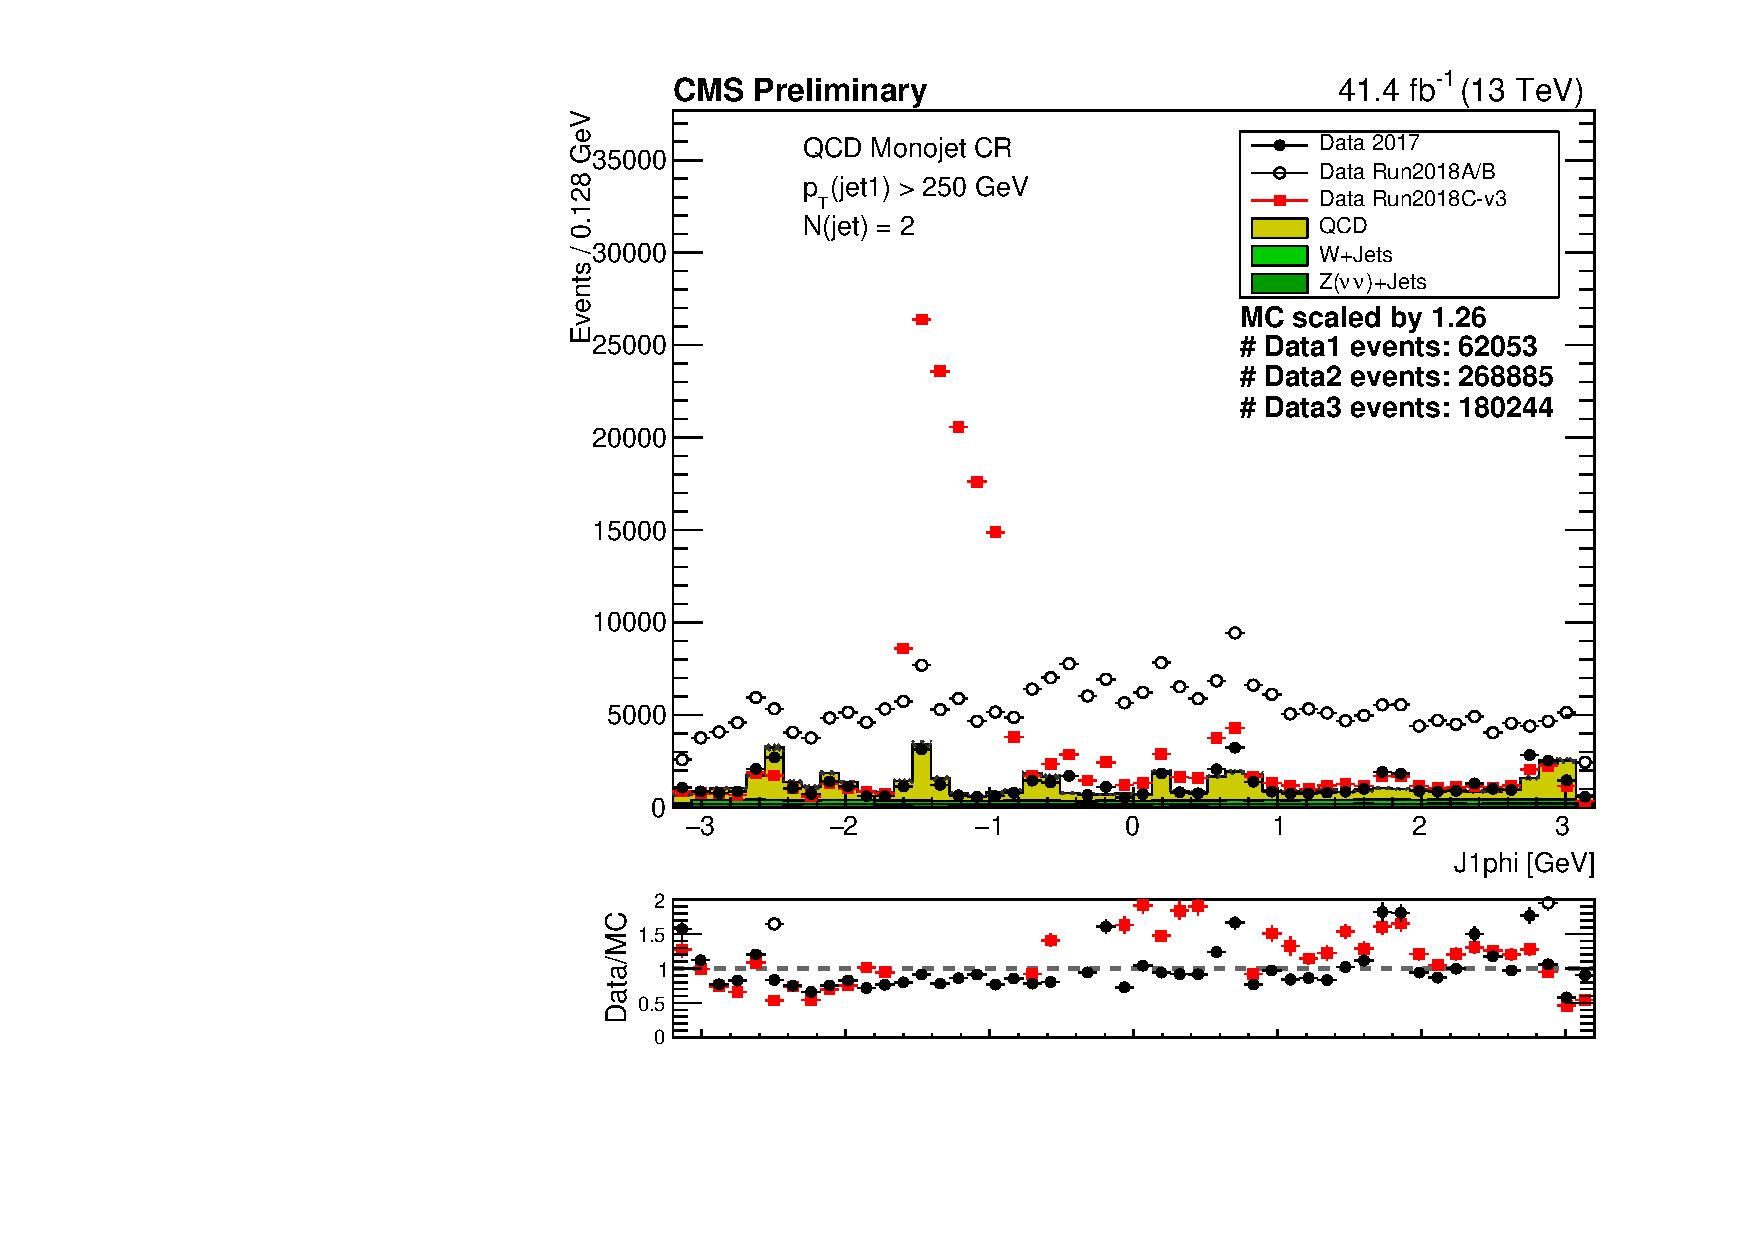
\includegraphics[width=0.48\textwidth]{figs/event_selection/hem_subleadjetphi.pdf} \\
    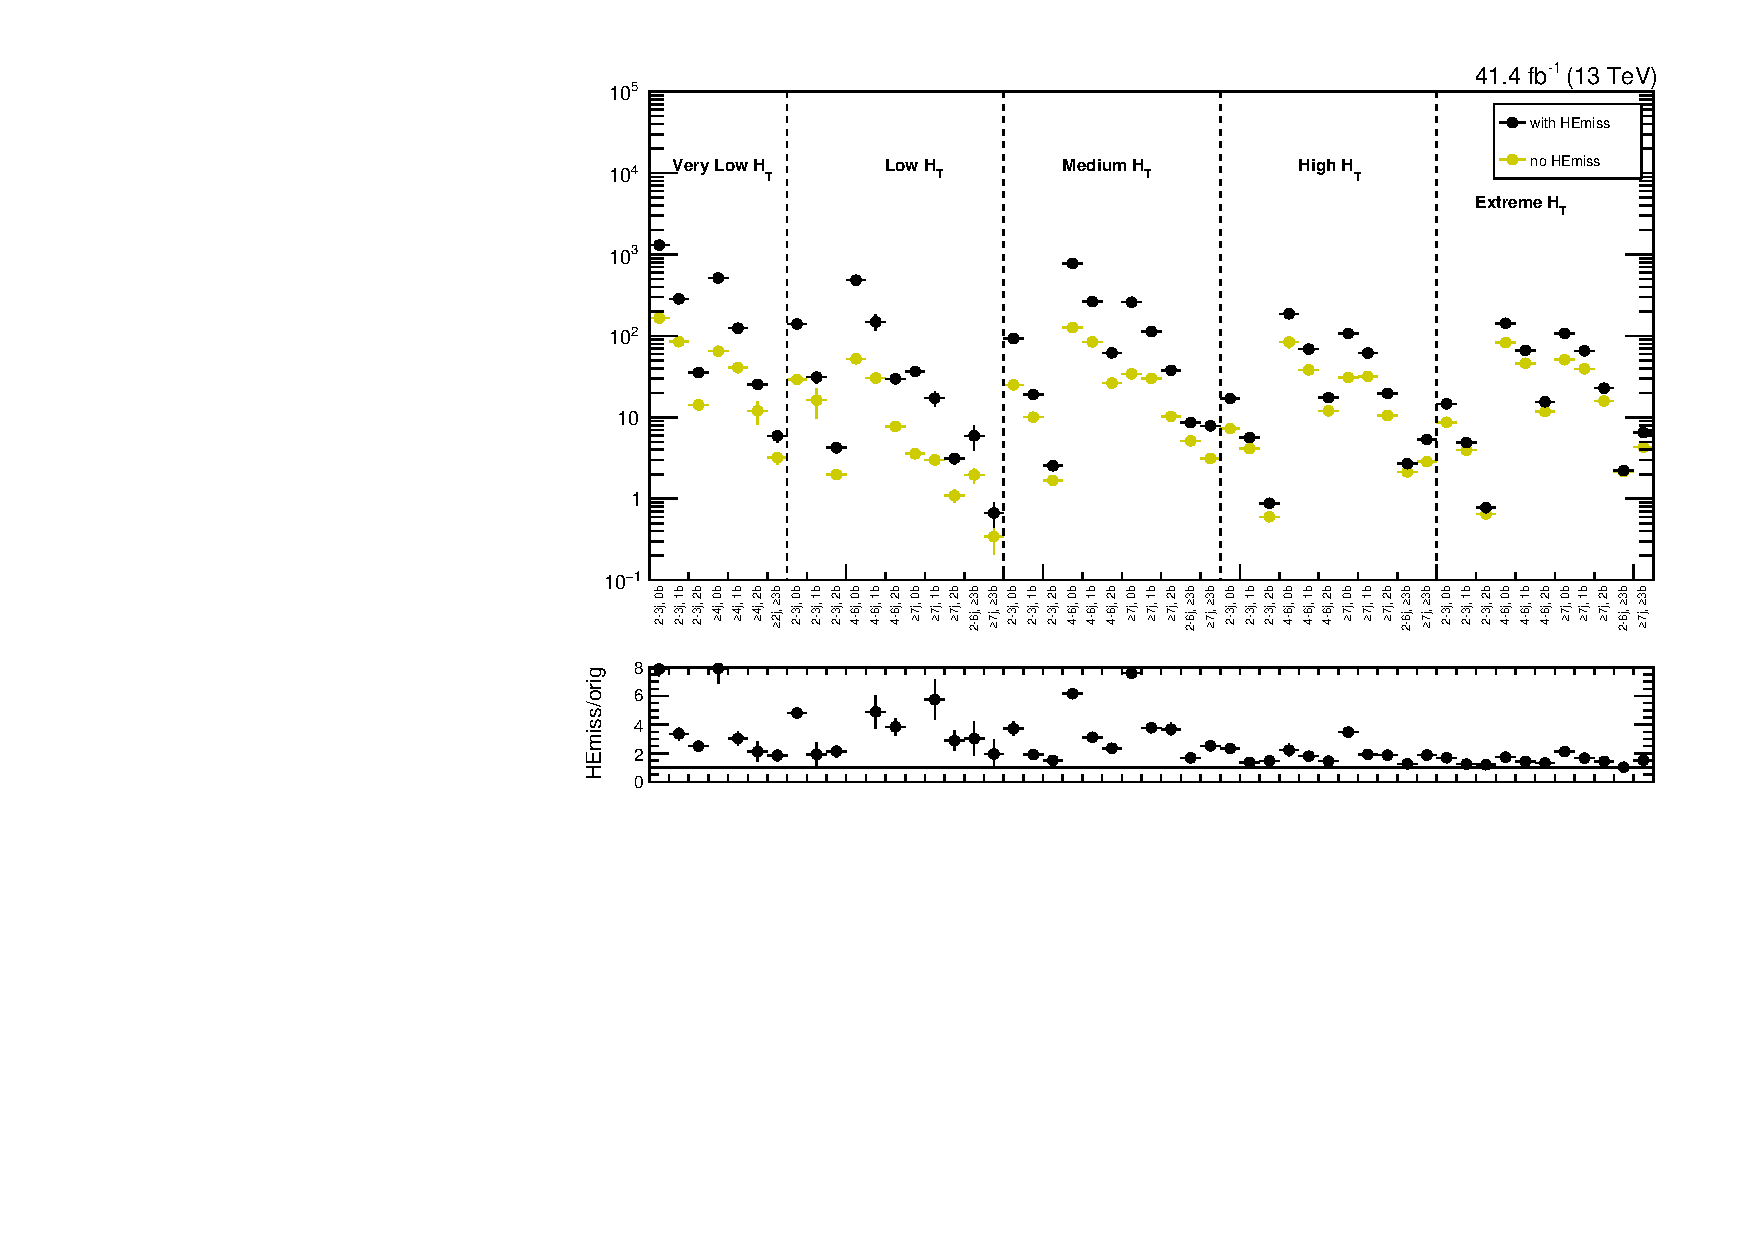
\includegraphics[width=0.70\textwidth]{figs/event_selection/mc_closure_sr.pdf}
    \caption{(top) Sub-leading jet $\eta$ and $\phi$ before and after the HEM issue.
      Black points are 2017, and are flat in $\phi$ and agree with MC. White
      points are early pre-HEM issue 2018 data, flat in $\phi$ but with 
      a uniform barrel-only excess due to an unrelated filter issue that was since fixed.
      Red points are post-HEM issue 2018 data, showing a clear excess in the HEM region
      $\eta\in[-4.7,-1.4]$, $\phi\in[-1.6,0.8]$. Dijet events that are otherwised 
      balanced but thathave a jet in
      the HEM region become imbalanced due to the lost energy.
      (bottom) Estimated effect of HEM issue on QCD signal region yields, found by 
      modifying Rebalance \& Smear templates with special response functions measured
      in HEM-emulated data. The issue causes up to an 8-fold increase in estimated
      background, and the effect is worst at low \Ht.
            }
    \label{fig:hem}
  \end{center}
\end{figure}
